%%%%%%%%%%%%%%%%%%%%%%%%%%%%%%%%%%%%%%%%%%%%%%%%%%%%%%%%%%
%%
%%      Prequantum Groupoid in Diffeology
%%      Part II: The General Case
%%
%%      Dec. 31, 2025
%%
%%      Patrick Iglesias-Zemmour
%%
%%%%%%%%%%%%%%%%%%%%%%%%%%%%%%%%%%%%%%%%%%%%%%%%%%%%%%%%%%

\documentclass[11pt,reqno,letterpaper,twoside]{amsart}

%%%%%%%%%%%%%%%%%%%%%%%%%%%%%%%%%%%%%%%%%%%%%%%%%%%%%%%%%%
%% MARK: - Macro file
%%
%%%%%%%%%%%%%%%%%%%%%%%%%%%%%%%%%%%%%%%%%%%%%%%%%%%%%%%%%%

\parindent 0mm
\parskip .5ex plus 2pt

\usepackage{amsmath}
\usepackage{amsbsy}
\usepackage{amssymb}
\usepackage{tikz-cd}
\usetikzlibrary{calc}
\tikzcdset{arrow style=tikz, diagrams={>={Straight Barb[scale=0.8]}}}

\usepackage{url}
\usepackage[margin=10pt,font=small,labelfont=bf, labelformat=simple, labelsep=endash]{caption}

\newtheoremstyle{articlestyle}% ⟨name⟩
{7pt}%  ⟨Space above⟩
{7pt}%  ⟨Space below⟩
{}%     ⟨Body font⟩
{0pt}%  ⟨Indent amount⟩
{\bf}%  ⟨Theorem head font⟩
{.\ }%  ⟨Punctuation after theorem head⟩
{0pt}%  ⟨Space after theorem head⟩
{}%     ⟨Theorem head spec (can be left empty, meaning ‘normal’)⟩

\theoremstyle{articlestyle}
\newtheorem{article}{}

\theoremstyle{plain}
\newtheorem{theorem}{Theorem}

\theoremstyle{definition}
\newtheorem{definition}{Definition}
\newtheorem{remark}{Remark}
\newtheorem{proposition}{Proposition}
\newtheorem{lemma}{Lemma}
\newtheorem{corollary}{Corollary}


\def\artlabel[#1]{\textbf{#1.}}
\newcommand{\widetext}[1]{\ \text{ #1 } \ }
\newcommand{\qtext}[1]{\quad\text{#1}\quad}

\newcommand{\RR}{\mathbf{R}}
\newcommand{\ZZ}{\mathbf{Z}}
\newcommand{\CC}{\mathbf{C}}
\newcommand{\TT}{\mathbf{T}}
\newcommand{\QQ}{\mathbf{Q}}
\newcommand{\HH}{\mathbf{H}}

\newcommand{\cB}{{\mathcal B}}
\newcommand{\cI}{{\mathcal I}}
\newcommand{\cY}{{\mathcal Y}}
\newcommand{\cG}{{\mathcal G}}
\newcommand{\blambda}{{\pmb{\lambda}}}

\newcommand{\fS}{{\frak S}}

\DeclareMathOperator{\PeriodsOf}{Periods}
\DeclareMathOperator{\comp}{comp}
\DeclareMathOperator{\Paths}{Paths}
\DeclareMathOperator{\Loops}{Loops}
\DeclareMathOperator{\Maps}{Maps}
\DeclareMathOperator{\Diff}{Diff}
\DeclareMathOperator{\Aut}{Aut}
\DeclareMathOperator{\Mor}{Mor}
\DeclareMathOperator{\Obj}{Obj}
\DeclareMathOperator{\pr}{pr}
\DeclareMathOperator{\src}{src}
\DeclareMathOperator{\trg}{trg}

% Fix for \ends conflict
\def\ends{\operatorname{ends}}

\DeclareMathOperator{\Ham}{Ham}
\DeclareMathOperator{\Ext}{Ext}
\DeclareMathOperator{\Hom}{Hom}
\DeclareMathOperator{\class}{class}
\DeclareMathOperator{\supp}{supp}

\DeclareMathOperator{\CHO}{\boldsymbol{\mathsf{K}}}
\newcommand{\Komega}{\CHO\!\omega}
\DeclareMathOperator{\Mid}{\big|}

\newcommand{\0}{\hat{0}}
\newcommand{\1}{\hat{1}}
\newcommand{\id}{\mathbf 1}
\newcommand{\U}{\mathrm{U}}
\newcommand{\T}{\mathrm{T}}
\newcommand{\D}{\mathrm{D}}
\newcommand{\dt}{d\!t}
\newcommand{\ds}{d\!s}
\newcommand{\df}{d\!f}

\newcommand{\Pomega}{\mathrm{P}_\omega}
\newcommand{\Tomega}{\mathrm{T}_\omega}
\newcommand{\Ttor}{\mathrm{T}_{\mathrm{tor}}}
\newcommand{\Psph}{\mathrm{P}_{\mathrm{sph}}}
\newcommand{\Phol}{\mathrm{P}_{\mathrm{hol}}}
\newcommand{\Ptor}{\mathrm{P}_{\mathrm{tor}}}
\newcommand{\paths}{\mathrm{paths}}
\newcommand{\quant}{\mathrm{quant}}
\newcommand{\tor}{\mathrm{tor}}
\newcommand{\sph}{\mathrm{sph}}
\newcommand{\surf}{\mathrm{surf}}
\newcommand{\loc}{\mathrm{loc}}

\newcommand{\vect}[1]{\begin{pmatrix}#1\end{pmatrix}} % usage : \vect{a \\ b \\...}

\usepackage{cfr-lm}

\usepackage[T1]{fontenc}
\usepackage[utf8]{inputenc}
\usepackage{microtype}
\usepackage[cal=scr,uppercase = upright, greekfamily = didot, greeklowercase = upright, utopia]{mathdesign}

\linespread{1.1}

\allowdisplaybreaks

%%%%%%%%%%%%%%%%%%%%%%%%%%%%%%%%%%%%%%%%%%%%%%%%%%%%%%%%%%
%%
%% MARK: - Begin Document
%%
%%%%%%%%%%%%%%%%%%%%%%%%%%%%%%%%%%%%%%%%%%%%%%%%%%%%%%%%%%

\begin{document}
  
  %%%%%%%%%%%%%%%%%%%%%%%%%%%%%%%%%%%%%%%%%%%%%%%%%%%%%%%%%%
  %% MARK: Title & Data
  %%%%%%%%%%%%%%%%%%%%%%%%%%%%%%%%%%%%%%%%%%%%%%%%%%%%%%%%%%
  
  \title[Geometric Quantization by Paths II]{Geometric Quantization by Paths \\ {\scriptsize Part II: The General Case}}
  
  \author{Patrick Iglesias-Zemmour}
  
  \address{Einstein Institute of Mathematics,
  The Hebrew University of Jerusalem,
  Campus Givat Ram,
  9190401 Israel.}
  \email{piz@math.huji.ac.il}
  \urladdr{http://math.huji.ac.il/~piz}
  \urladdr{https://github.com/p-i-z/Diffeology-Archives}
  
  \thanks{The author thanks the Hebrew University of Jerusalem, Israel, for his continuous academic support. He is also grateful for the stimulating discussions and assistance provided by the AI assistant Gemini (Google).
  \\
  The \TeX\ source of this paper is available at the GitHub PIZ-Diffeology Archive: \url{https://github.com/p-i-z/Diffeology-Archives}.}
  
  \date{Typeset Jan. Sun. 4, 2026 (Added "Elementary vs composite systems", "The Intrinsic Action Principle")}
  
  \subjclass[2020]{Primary 53D50, 58A05; Secondary 22A22, 55R65, 58A10}
  \keywords{Diffeology, Geometric Quantization, Prequantum Groupoid, Closed 2-forms, Parasymplectic Spaces, Paths, Loops}
  
  \dedicatory{To the memory of Jean-Marie Souriau, who once asked me: \\ ``Quoi de neuf en diffeolog'y ?''}
  
  %%%%%%%%%%%%%%%%%%%%%%%%%%%%%%%%%%%%%%%%%%%%%%%%%%%%%%%%%%
  %% MARK: Abstract
  %%%%%%%%%%%%%%%%%%%%%%%%%%%%%%%%%%%%%%%%%%%%%%%%%%%%%%%%%%
  
  \begin{abstract}
    \noindent In Part I, we established the construction of the prequantum groupoid for simply connected spaces.
    This second part extends the theory to \emph{arbitrary connected parasymplectic diffeological spaces} $(X, \omega)$.
    We identify the obstruction to the existence of the prequantum groupoid as the non-additivity of the integration of the prequantum form $\Komega$ on the space of loops.
    
    \noindent By defining a \emph{Total Group of Periods} $\Pomega$ directly on the space of paths, which absorbs the periods arising from the algebraic relations of the fundamental group, we construct a prequantum groupoid $\TT_\omega$ with connected isotropy isomorphic to the torus of periods $T_\omega = \RR/\Pomega$.
    
    \noindent Furthermore, we propose that this groupoid $\TT_\omega$ constitutes the \emph{Quantum System} itself.
    The classical space $X$ is embedded as the \emph{Skeleton} of units, surrounded by a \emph{Quantum Fog} of non-identity morphisms.
    We prove that the group of automorphisms of the Quantum System is isomorphic to the group of symmetries of the Dynamical System, $\Diff(X, \omega)$.
  \end{abstract}
  
  \maketitle
  
  %%%%%%%%%%%%%%%%%%%%%%%%%%%%%%%%%%%%%%%%%%%%%%%%%%%%%%%%%%
  %% MARK: Introduction
  %%%%%%%%%%%%%%%%%%%%%%%%%%%%%%%%%%%%%%%%%%%%%%%%%%%%%%%%%%
  
  \section*{\textsc{\textbf{Introduction}}}
  
  This paper is the continuation of the author's work on geometric quantization by path \cite{PIZ25a} within the framework of diffeology \cite{PIZ13}.
  In Part I,
  we established the construction of the prequantum groupoid $\TT_\omega$ for connected and simply connected parasymplectic spaces $(X,\omega)$.
  We showed that this object, defined as a quotient of the space of paths, encodes the prequantum geometry more naturally than the traditional principal bundle approach.
  In particular,
  the quantum phase emerged intrinsically as the isotropy group of the groupoid,
  isomorphic to the torus of periods.
  
  However,
  the assumption of simple connectedness is restrictive.
  Many physically relevant systems,
  such as the torus or surfaces of higher genus,
  are not simply connected.
  In these cases,
  the geometry of the space $X$ introduces new periods
  ---surfacic periods---
  that are not captured by the spherical or toric cycles alone.
  A naive application of the previous construction would fail to produce a connected isotropy group,
  leading to a disconnected phase structure that contradicts physical intuition.
  
  In this Part II,
  we extend the construction to arbitrary connected diffeological spaces.
  Our strategy relies on a direct \emph{Path Approach}:
  we identify the obstruction to the additivity of the prequantum action directly within the space of loops of $X$.
  This obstruction is measured by a cocycle defined on the fundamental group of the space.
  By incorporating the values of this cocycle on the group relations into the definition of the \emph{Total Group of Periods} $\Pomega$,
  we ensure that the prequantum structure closes on the quotient \emph{torus of periods} $\Tomega = \RR/\Pomega$.
  The only requirement for a non-trivial quantization is that this group of periods $\Pomega$ differs from $\RR$,
  or equivalently,
  that the torus $\Tomega$ is not reduced to a point.\footnote{In diffeology, a subset $A \subset B$ is discrete if it carries the discrete diffeology (locally constant plots). For a subgroup of $\RR$, being discrete is equivalent to being a strict subgroup ($P \neq \RR$). Thus, we use "discrete" and "$\neq \RR$" interchangeably.}
  
  This generalization leads us to a broader conceptual proposal.
  We suggest that the prequantum groupoid $\TT_\omega$ constitutes the \emph{Quantum System} itself.
  The classical space $X$ sits inside it as the \emph{Skeleton} of units,
  surrounded by a \emph{Quantum Fog} of non-unit morphisms.
  We show that the symmetries of the classical system lift fully and faithfully to this structure,
  satisfying the Dirac axioms for quantization naturally.
  
  This perspective resolves a long-standing ambiguity regarding the status of conserved quantities in geometrically non-trivial systems.
  We show that the "paths moment map,"
  introduced in our previous work on the moment map in diffeology \cite{PIZ10},
  is precisely the intrinsic moment map of the quantum groupoid.
  The holonomy group $\Gamma$,
  classically viewed as an obstruction to the existence of single-valued observables on the space of motions (violating Souriau's principle of the moment map),
  is reinterpreted here as a signature of strictly quantum geometrical features.
  The classical moment map is then the shadow of this "absolute quantum moment map".
  The groupoid framework thus accommodates systems like the Aharonov-Bohm effect without pathology,
  treating multi-valued classical quantities as single-valued quantum morphisms.
  
  \subsection*{The Missing Link to Feynman's Integral}
  This construction offers a rigorous geometric resolution to the intuition underlying Feynman's path integral.
  Feynman's approach seeks to extract quantum amplitudes by summing over the space of all paths,
  relying on the interference of the phase factor $\exp(i S/\hbar)$ to isolate physical contributions.
  
  Our approach reveals that geometric quantization is the dual operation:
  rather than \emph{integrating} over the "noise" of the infinite-dimensional path space, we \emph{quotient it out}.
  The equivalence relation defining the groupoid $\TT_\omega$ identifies precisely those paths that possess the same symplectic action\footnote{Strictly speaking, one should write “parasymplectic action.” The word symplectic is not used in its strict and rigorous sense, but only to give a flavor of the context.} (modulo periods).
  
  The prequantum groupoid is,
  therefore,
  the geometric \emph{reification} of the path integral's phase structure.
  It implies that there is no "hidden physics" in the Feynman approach that is absent from the Dirac-Souriau program;
  the information is identical, provided one looks for it in the correct place:
  not on the base space $X$,
  but on the "floor above"
  ---the space of paths $\Paths(X)$.
  The groupoid provides the rigorous geometric container for the path integral,
  free from the measure-theoretic difficulties of functional integration.
  
  \subsection*{A Note on the Diffeological Framework}
  It is crucial to emphasize that throughout this work,
  all mathematical objects
  ---the base space $X$, the space of paths $\Paths(X)$, the group of periods $\Pomega$, and the resulting groupoid $\TT_\omega$---
  are treated strictly as \emph{diffeological spaces}.
  We make no assumptions regarding their status as manifolds,
  infinite-dimensional manifolds,
  or Lie groups.
  
  The operations of taking quotients (such as the torus of periods $\Tomega = \RR/\Pomega$ or the groupoid space of morphisms $\cY$) and forming functional spaces (such as $\Paths(X)$) are internal to the category of diffeology.
  They require no topological or regularity conditions
  ---such as the topological discreteness of the period group or the local Euclidean nature of the quotient---
  to yield well-defined smooth structures.
  This framework allows us to treat standard symplectic manifolds,
  general parasymplectic spaces,
  singular quotient spaces,
  and infinite-dimensional loop spaces within a single,
  uniform geometric theory.
  
  %%%%%%%%%%%%%%%%%%%%%%%%%%%%%%%%%%%%%%%%%%%%%%%%%%%%%%%%%%
  %% MARK: Section I: The Group and the Torus of Periods
  %%%%%%%%%%%%%%%%%%%%%%%%%%%%%%%%%%%%%%%%%%%%%%%%%%%%%%%%%%
  
  \section{\textsc{\textbf{The Group and the Torus of Periods}}}
  \label{sec:GroupAndTorusOfPeriods}
  
  The torus of periods,
  quotient of the real line $\RR$ by the group of periods $\Pomega$,
  plays a fundamental role in geometric quantization.
  In the general case,
  $\Pomega$ involves three sources of periods: the \emph{spherical periods} (from contractible spheres),
  the \emph{toric periods} (from the geometry of loop components),
  and the \emph{surfacic periods} (from the non-commutative homotopy of $X$).
  
  \begin{article}\artlabel[The Toric Periods]
    Let $(X,\omega)$ be a connected parasymplectic diffeological space.
    We recall the chain-homotopy operator $\CHO: \Omega^k(X) \to \Omega^{k-1}(\Paths(X))$.
    For $\omega \in \Omega^2(X)$,
    let $\Komega = \CHO(\omega) \in \Omega^1(\Paths(X))$.
    
    Since $d\omega = 0$,
    the restriction of $\Komega$ to the space of loops $\Loops(X)$ is closed.
    We decompose the loop space into its connected components:
    $$
      \Loops(X) = \coprod_{i \in \pi_0(\Loops(X))} L_i.
      $$
    On each component $L_i$,
    the restriction of $\Komega$ defines a local group of periods:
    $$
      P_i = \left\{ \int_\sigma \Komega \mid \sigma \in \Loops(L_i) \right\} \subset \RR.
      $$
    We define the \emph{Group of Toric Periods} $\Ptor$ as the subgroup of $\RR$ generated by the union of all local periods:
    $$
      \Ptor = \left\langle \bigcup_{i} P_i \right\rangle.
      $$
    We assume $\Ptor$ is discrete.
    The quotient $\Ttor = \RR/\Ptor$ is the \emph{Torus of Toric Periods};
    it comes equipped with its canonical volume forms $\theta_{\tor}$\,:
    $$
      \T_\tor = \RR/P_\tor
      \qtext{and}
      \theta_\tor \in \Omega^1(\T_\tor)
      \qtext{such that} \pi_\tor^*(\theta_\tor) = \dt,
      $$
  \end{article}
  
  \begin{article}\artlabel[The Group of Indices]
    To capture the homotopy of $X$,
    we must structure the set of components.
    Let us fix a base point $x_0 \in X$.
    We consider the subspace of based loops $\Loops(X, x_0)$.
    
    The set of connected components of $\Loops(X, x_0)$ forms the fundamental group of $X$.
    Let $\cI = \pi_0(\Loops(X, x_0))$.
    The concatenation of loops induces a group operation on $\cI$,
    denoted by $*$.
    
    We choose a \emph{basis of loops} $\cB = \{ \ell_i \}_{i \in \cI}$ such that:
    \begin{enumerate}
      \item For each $i \in \cI$, $\ell_i \in \Loops(X, x_0)$ belongs to the component $i$.
      \item For the identity element $1 \in \cI$,
      we choose the constant loop: $\ell_1 = \hat{x}_0$.
    \end{enumerate}
  \end{article}
  
  \begin{article}\artlabel[The Integration Function]
    We define an integration function $\phi: \Loops(X, x_0) \to \Ttor$ component-wise.
    For any loop $\ell$ in the component $i \in \cI$:
    $$
      \phi(\ell) = \pi_{\tor} \left( \int_{\ell_i}^\ell \Komega \right) \in \Ttor,
      $$
    where $\pi_{\tor}: \RR \to \Ttor$ is the projection.
    The integral is well-defined in $\Ttor$ because any two paths from $\ell_i$ to $\ell$ within $L_i$ differ by a period in $P_i \subset \Ptor$.
    By construction,
    this function satisfies the differential relation:
    $$
      \phi^*(\theta_\tor) = \Komega \restriction \Loops(X, x_0).
      $$
  \end{article}
  
  \begin{article}\artlabel[The Surfacic Cocycle]
    The function $\phi$ measures the symplectic action relative to the basis $\cB$.
    However,
    $\phi$ is generally not a homomorphism with respect to loop concatenation.
    
    Consider two loops $\ell \in L_i$ and $\ell' \in L_j$.
    The integral defining $\phi(\ell \vee \ell')$ decomposes geometrically into two steps:
    first from the basis loop $\ell_{i*j}$ to the concatenation of bases $\ell_i \vee \ell_j$,
    and then from $\ell_i \vee \ell_j$ to the target $\ell \vee \ell'$.
    $$
      \int_{\ell_{i*j}}^{\ell \vee \ell'} \Komega = \int_{\ell_{i*j}}^{\ell_i \vee \ell_j} \Komega + \int_{\ell_i \vee \ell_j}^{\ell \vee \ell'} \Komega.
      $$
    Using the property of integrating concatenations over homotopies established in Part I,
    the second term splits into the sum of individual integrals:
    $$
      \int_{\ell_i \vee \ell_j}^{\ell \vee \ell'} \Komega = \int_{\ell_i}^{\ell} \Komega + \int_{\ell_j}^{\ell'} \Komega.
      $$
    Consequently,
    we obtain the fundamental relation:
    $$
      \phi(\ell \vee \ell') = \tau(i,j) + \phi(\ell) + \phi(\ell'),
      $$
    where the defect is measured by the \emph{surfacic cocycle} $\tau: \cI \times \cI \to \Ttor$:
    $$
      \tau(i,j) = \pi_{\tor} \left( \int_{\ell_{i*j}}^{\ell_i \vee \ell_j} \Komega \right).
      $$
    
    \begin{figure}[t]
      \centering
      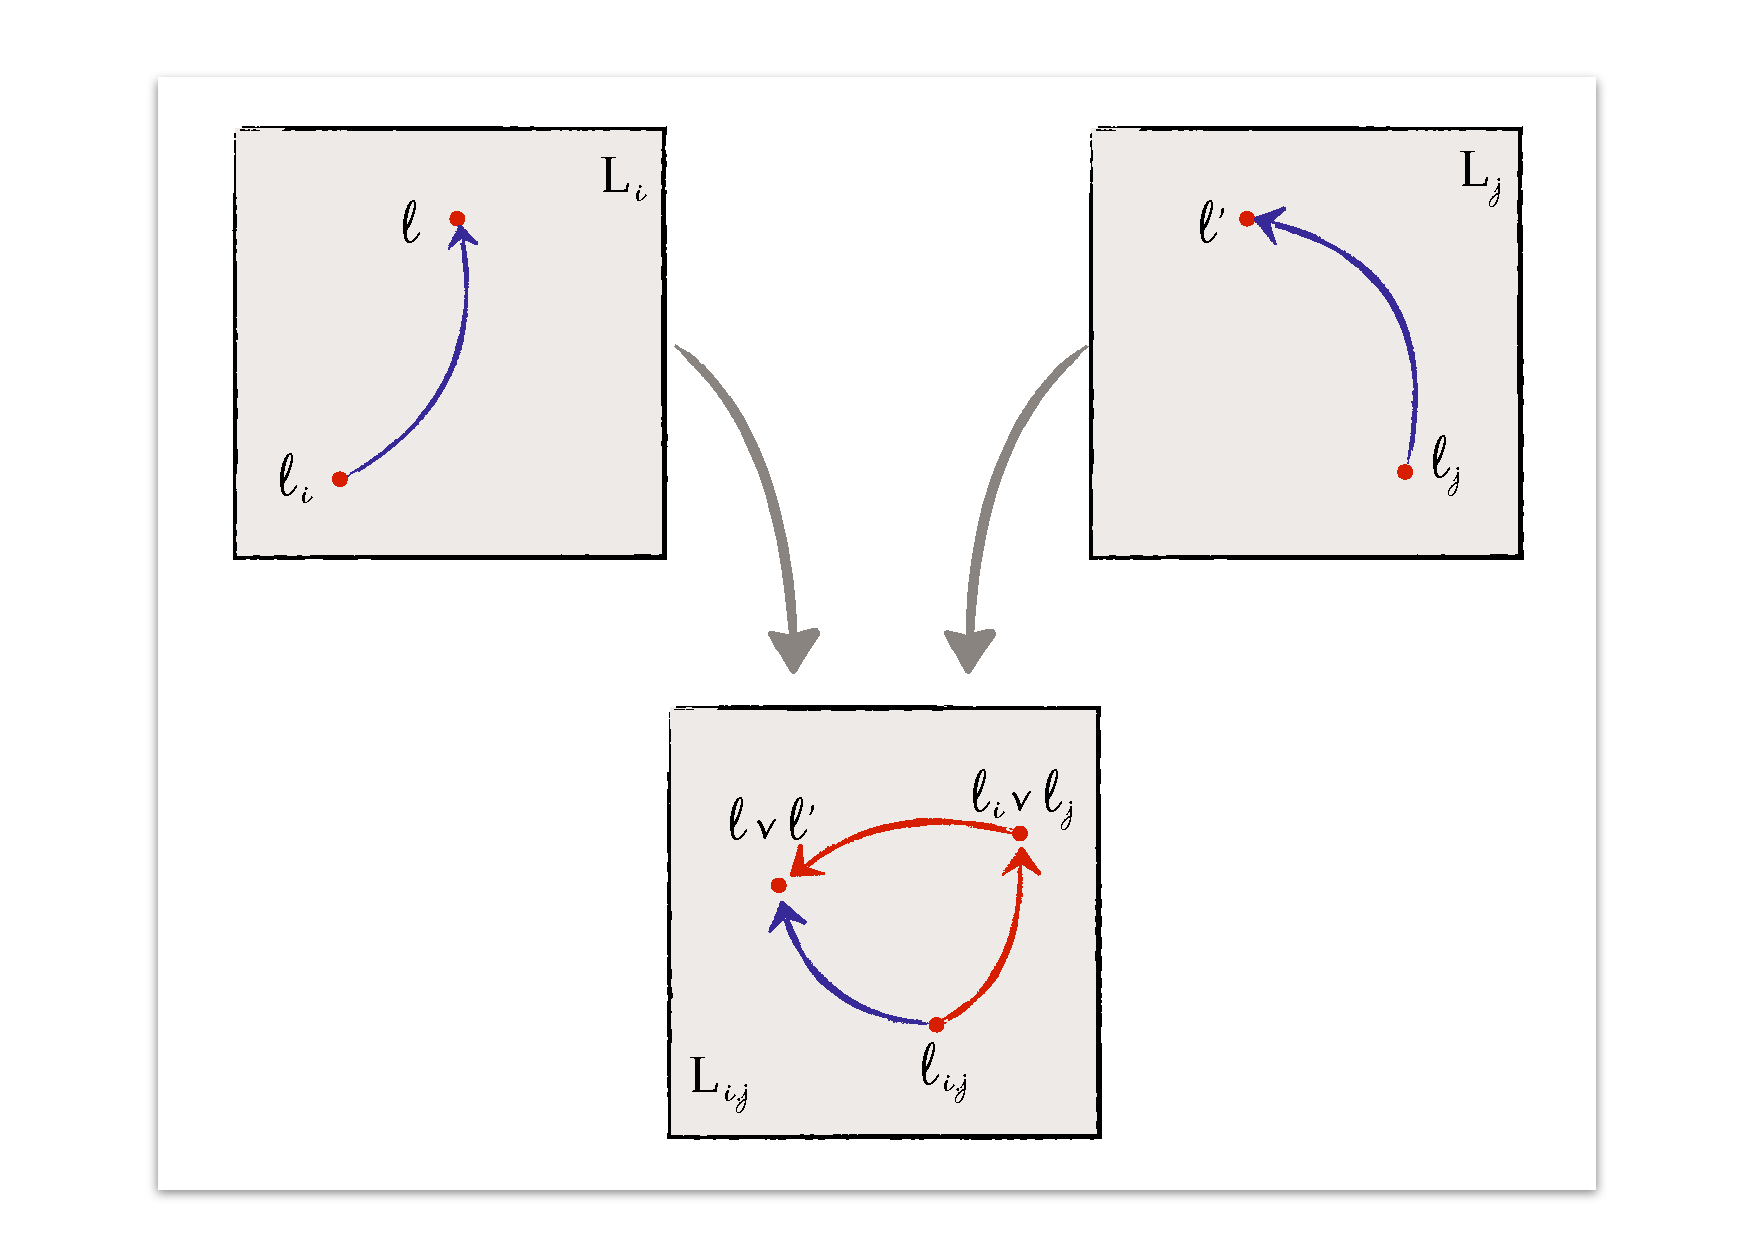
\includegraphics[width=0.75\textwidth]{Figures/fig-lij.pdf}
      \caption{\small\textbf{The Construction of the Surfacic Cocycle.}
      The integration path from the basis loop $\ell_{i*j}$ to $\ell \vee \ell'$ decomposes into the cocycle path (from $\ell_{i*j}$ to $\ell_i \vee \ell_j$) and the concatenation of individual paths.
      Summing the integrals yields $\phi(\ell \vee \ell') = \tau(i,j) + \phi(\ell) + \phi(\ell')$.}
      \label{fig:cocycle}
    \end{figure}
    
    \begin{proposition}[The Surfacic Cocycle]
      The map $\tau$ is a group $2$-cocycle of $\cI$ with values in $\Ttor$.
      For any $i,j,k \in \cI$:
      $$
        \tau(i,j) + \tau(i*j, k) = \tau(i, j*k) + \tau(j,k).
        $$
    \end{proposition}
    
    \begin{proof}
      The proof follows from the associativity of loop concatenation up to homotopy.
      We evaluate the integration function $\phi$ on the triple concatenation $\ell_i \vee \ell_j \vee \ell_k$ in two ways.
      First, as $(\ell_i \vee \ell_j) \vee \ell_k$, applying the decomposition formula twice yields terms involving $\tau(i,j)$ and $\tau(i*j, k)$.
      Second, as $\ell_i \vee (\ell_j \vee \ell_k)$, yielding terms involving $\tau(j,k)$ and $\tau(i, j*k)$.
      Since the two concatenation orders are homotopic (associativity), and the integral of $\Komega$ is invariant under fixed-ends homotopy (modulo $\Ptor$), the two expansions must be equal.
      Canceling the individual terms $\phi(\ell_i) + \phi(\ell_j) + \phi(\ell_k)$ leaves the cocycle identity.
    \end{proof}
    
    The value $\tau(i,j) - \tau(j,i)$ represents the symplectic area of the commutator $[\ell_i, \ell_j]$,
    which corresponds to the curvature of the bundle over the surface defined by the commutator.
  \end{article}
  
  \begin{article}\artlabel[The Central Extension]
    The cocycle $\tau$ defines a group extension $\tilde{\Gamma}$ of the fundamental group $\cI$ by the torus $\Ttor$.
    The elements of $\tilde{\Gamma}$ are pairs $(i, u) \in \cI \times \Ttor$ with the multiplication law:
    $$
      (i, u) \cdot (j, v) = (i*j, u + v + \tau(i,j)).
      $$
    This extension is \emph{central}:
    In the general theory of group extensions, the multiplication involves an action $\rho$ of the base on the fiber: $u + \rho(i)(v) + \tau(i,j)$.
    Here, the formula simply sums $u+v$, implying that the action $\rho$ is the identity.
    Consequently, elements of the fiber $(1, a)$ commute with all elements of $\tilde{\Gamma}$:
    $$
      (i, u) \cdot (1, a) = (i, u+a) = (1, a) \cdot (i, u).
      $$
    This algebraic fact reflects the physical principle that the nature of the quantum phase (the torus $\Ttor$) is intrinsic and does not change as one moves around the fundamental group of the space.
  \end{article}
  
  \begin{article}\artlabel[The Total Group of Periods]
    \label{art:totalgroupperiods}
    We now define the total group of periods $\Pomega$ intrinsically,
    absorbing the periods generated by the non-trivial homotopy.
    
    Let $F(\cI)$ be the free group generated by the elements of $\cI$.
    An element of $F(\cI)$,
    a word $w = (i_1, \dots, i_k) \in F(\cI)$,
    is a \emph{relation} if the product $i_1 * \dots * i_k = 1$ in $\cI$.
    Let $\mathcal{R}$ be the set of relations.
    
    Recall that the fundamental group $\cI \simeq \pi_1(X, x_0)$ is isomorphic to the quotient of the free group $F(\cI)$ by the normal subgroup generated by $\mathcal{R}$.
    Geometrically,
    a relation $w$ corresponds to a specific concatenation of basis loops that is contractible in $X$.
    While such a loop is homotopically trivial,
    the symplectic area it encloses (measured by the cocycle) is not necessarily zero.
    
    We define the \emph{Accumulated Cocycle} $\mathcal{T}$ using the universal property of free groups.
    Let $\sigma: \cI \to \tilde{\Gamma}$ be the set-theoretic section defined by $\sigma(i) = (i, 0)$.
    By the universal property, $\sigma$ extends uniquely to a group homomorphism $\Psi: F(\cI) \to \tilde{\Gamma}$.
    
    Since $\pi \circ \Psi(i) = i$ for all generators, the homomorphism $\Psi$ lifts the projection $p: F(\cI) \to \cI$.
    Consequently, $\Psi$ maps the kernel of $p$ (the relations $\mathcal{R}$) into the kernel of $\pi$ (the fiber $\Ttor$).
    
    Since a relation $w$ represents a contractible loop in $X$,
    it bounds a surface.
    The accumulated cocycle $\mathcal{T}(w)$ measures the symplectic area of this surface.
    
    For any relation $w \in \mathcal{R}$,
    we define $\mathcal{T}(w)$ by the condition:
    $$
      \Psi(w) = (1, \mathcal{T}(w)).
      $$
    This value $\mathcal{T}(w) \in \Ttor$ represents the total phase accumulated by traversing the loop corresponding to the relation $w$.
    
    \begin{definition}[Total Group of Periods]
      Let $H_\surf \subset \Ttor$ be the subgroup generated by the values $\{ \mathcal{T}(w) \mid w \in \mathcal{R} \}$.
      The \emph{Total Group of Periods} is the preimage:
      $$
        \Pomega = \pi_{\tor}^{-1}(H_\surf) \subset \RR.
        $$
    \end{definition}
    
    We assume $\Pomega \neq \RR$.
    The quotient $\Tomega = \RR/\Pomega$ is the \emph{Total Torus of Periods}.
    By construction,
    the cocycle $\tau$ vanishes when projected to $\Tomega$, ensuring the additivity required for the groupoid construction.
    
    \textbf{Remark.}~(Minimality).
    This construction represents the \emph{minimal} quantization condition.
    The group $\Pomega$ is the smallest subgroup of $\RR$ containing $\Ptor$ that absorbs the symplectic areas of the fundamental relations.
    Any smaller group would fail to trivialize the cocycle $\tau$ in the quotient,
    leaving the integration function $\psi$ non-additive and the groupoid structure ill-defined.
    
    \begin{proposition}[Independence of the Periods]
      \label{art:independenceperiods}
      The Total Group of Periods $\Pomega$ is independent of the choice of the basis of loops $\cB = \{ \ell_i \}_{i \in \cI}$,
      and of their base point $x_0 \in X$.
    \end{proposition}
    
  \end{article}
  
  \begin{proof}
    We prove that the accumulated cocycle $\mathcal{T}(w)$ is independent of the basis modulo $\Ptor$ by a pure geometrical argument.
    
    1.~\emph{Construction of the Deformation Path.}
    Let $\cB = \{ \ell_j \}$ and $\cB' = \{ \ell'_j \}$ be two bases of loops at $x_0$.
    For each index $j \in \cI$, let $\eta_j$ be a path in $\Loops(X, x_0)$ connecting the old basis loop to the new one:
    $$
      \eta_j(0) = \ell_j \qtext{and} \eta_j(1) = \ell'_j.
      $$
    Let $w = (i_1, \dots, i_k)$ be a relation, meaning the product $i_1 * \dots * i_k = 1$ in $\pi_1(X, x_0)$.
    We define the path $H$ in $\Loops(X, x_0)$ connecting the composite loops of the two bases.
    The construction is defined by the concatenation of the loops in $X$:
    $$
      H(s) = \eta_{i_1}(s) \vee \eta_{i_2}(s) \vee \dots \vee \eta_{i_k}(s).
      $$
    Since $w$ is a relation, for every $s \in [0,1]$, the concatenation $H(s)$ is a loop in $X$ based at $x_0$ (homotopic to the constant loop).
    Thus, $H$ is a well-defined path in the functional space $\Loops(X, x_0)$ from $L_w = \ell_{i_1} \vee \dots \vee \ell_{i_k}$ to $L'_w = \ell'_{i_1} \vee \dots \vee \ell'_{i_k}$.
    
    2.~\emph{The Cycle in Loop Space.}
    The accumulated cocycle $\mathcal{T}(w)$ is defined by the integral from the identity loop $\ell_1$ (constant at $x_0$) to $L_w$.
    $$
      \mathcal{T}(w) \equiv \int_{\ell_1}^{L_w} \Komega \pmod{\Ptor}.
      $$
    Similarly for the second basis:
    $$
      \mathcal{T}'(w) \equiv \int_{\ell'_1}^{L'_w} \Komega \pmod{\Ptor}.
      $$
    Consider the closed cycle $\Gamma$ in $\Loops(X)$ formed by the path defining $\mathcal{T}(w)$, followed by $H$, and closed by the inverse of the path defining $\mathcal{T}'(w)$.
    (Note that $\ell_1 = \ell'_1 = \hat{x}_0$).
    The integral over this cycle is a toric period:
    $$
      \int_{\ell_1}^{L_w} \Komega + \int_{L_w}^{L'_w} \Komega - \int_{\ell'_1}^{L'_w} \Komega \equiv 0 \pmod{\Ptor}.
      $$
    Substituting the terms, we isolate the difference:
    $$
      \mathcal{T}(w) - \mathcal{T}'(w) \equiv - \int_H \Komega \pmod{\Ptor}.
      $$
    
    3.~\emph{The Swapping Argument.}
    We calculate $\int_H \Komega$ explicitly to show it belongs to $\Ptor$.
    The path $H$ is represented by a plot $\Phi: \RR^2 \to X$,
    defined by $\Phi(s,t) = H(s)(t)$.
    Here $s$ is the homotopy parameter (the path variable) and $t$ is the loop parameter.
    Using the definition of $\Komega$:
    \begin{multline*}
      \int_H \Komega = \int_0^1 \Komega(H)_s(1) \ds
      = \int_0^1 \left[\int_0^1 \omega(\Phi)_{s \choose t} \left( \vect{1 \\ 0}, \vect{0 \\ 1 } \right) \dt \right] \ds \\
      = \int_0^1\int_0^1 \omega(\Phi)_{s \choose t} \left( \vect{1 \\ 0}, \vect{0 \\ 1 } \right) \ds\, \dt
      = - \int_0^1\int_0^1 \omega(\Phi)_{s \choose t} \left( \vect{0 \\ 1}, \vect{1 \\ 0 } \right) \dt\, \ds.
    \end{multline*}
    We swap the parameters to interpret this as an integral over a path $\tilde{H}$ in the transverse direction: $\tilde{H}(t)(s) = \Phi(s,t)$.
    Here, $t$ becomes the path variable and $s$ the loop variable.
    Thus:
    $$
      \int_H \Komega = - \int_{\tilde{H}} \Komega.
      $$
    We check the boundary conditions of $\tilde{H}$:
    \begin{itemize}
      \item At $t=0$: $\tilde{H}(0)$ is the path $s \mapsto \Phi(s,0)$.
      Since all loops are based at $x_0$,
      $\Phi(s,0) = x_0$. Thus $\tilde{H}(0) = \hat{x}_0$.
      \item At $t=1$:
      Similarly, $\Phi(s,1) = x_0$,
      so $\tilde{H}(1) = \hat{x}_0$.
    \end{itemize}
    Since $\tilde{H}$ starts and ends at the constant loop,
    it is a closed loop in the space $\Loops(X)$.
    Therefore,
    its integral is a toric period:
    $$
      \int_{\tilde{H}} \Komega \in \Ptor.
      $$
    This implies $\int_H \Komega \in \Ptor$.
    Consequently, $\mathcal{T}(w) = \mathcal{T}'(w)$ in $\Tomega$.
    
    4.~\emph{Independence from the Basepoint.}
    Let $x_1$ be another basepoint and $c$ a path from $x_1$ to $x_0$.
    The change of basepoint induces an isomorphism on the fundamental group by conjugation,
    mapping a loop $\ell$ based at $x_0$ to the loop $L = c \vee \ell \vee \bar c$ based at $x_1$.
    We show that $\phi(L) = \phi(\ell)$.
    
    Let $c_s$ be the path $t \mapsto c(s + t(1-s))$, which retracts the path $c$ to the constant path at point $x_0$ as $s$ goes from $0$ to $1$.
    Consider the homotopy $\sigma: s \mapsto c_s \vee \ell \vee \bar c_s$ in $\Loops(X)$.
    This homotopy connects the conjugated loop $L$ (at $s=0$) to the original loop $\ell$ (at $s=1$, since $c_1$ is the constant path at $x_0$).
    The difference in the values of $\phi$ is the integral of $\Komega$ along this homotopy:
    $$
      \phi(L) - \phi(\ell) = \int_\sigma \Komega = \int_{s \mapsto c_s} \Komega + \int_{s \mapsto \ell} \Komega + \int_{s \mapsto \bar c_s} \Komega.
      $$
    This integral decomposes into three terms corresponding to the three segments of the concatenated path $\sigma \in \Paths(\Loops(X))$.
    The central term vanishes because it is the integration of $\Komega$ on the constant path $s \mapsto \ell$.
    The term for the segment $s \mapsto c_s$ involves integrating $\omega$ over the map $\sigma(s)(t) = c_s(t)$.
    Since $\sigma$ factors through the smooth curve $c$,
    that is,
    a $1$-plot,
    this term vanishes identically.
    The same applies to the segment $\bar c_s$.
    Thus, $\int_\sigma \Komega = 0$.
    
    It follows that $\phi$ is invariant under conjugation.
    This fundamental invariance implies that the surfacic cocycle $\tau$ is itself invariant (as it is defined via $\phi$ on loops),
    and consequently,
    the Total Group of Periods $\Pomega$ is a canonical invariant of the parasymplectic space $(X, \omega)$, independent of the basepoint.
  \end{proof}
  
  \textbf{Remark.}(~On the Invariance)
  Geometrically, this result relies on the fact that the deformation of a relation sweeps out a closed surface (a sphere or a torus) in $X$.
  Algebraically, this corresponds to the fact that the variation of the accumulated cocycle is a coboundary that vanishes on cycles (relations) modulo the periods.
  The definition of $\Pomega$ ensures exactly that these geometric "bubbles" do not obstruct the definition of the groupoid.
  
  %%%%%%%%%%%%%%%%%%%%%%%%%%%%%%%%%%%%%%%%%%%%%%%%%%%%%%%%%%
  %% MARK: Section II: The Chasles Cocycle
  %%%%%%%%%%%%%%%%%%%%%%%%%%%%%%%%%%%%%%%%%%%%%%%%%%%%%%%%%%
  
  \section{\textsc{\textbf{The Chasles Cocycle}}}
  \label{sec:ChasleCocycle}
  
  With the Total Torus of Periods $\Tomega = \RR/\Pomega$ established,
  we can now define a global integration function on the entire space of loops $\Loops(X)$.
  This function will serve as the foundation for the Chasles cocycle.
  
  \begin{article}\artlabel[The Global Integration Function]
    Let $\pi_\omega: \RR \to \Tomega$ be the projection.
    We define the function $\psi: \Loops(X) \to \Tomega$ component-wise.
    For any loop $\ell$ belonging to the connected component $L_i$ (indexed by $i \in \cI$),
    we set:
    $$
      \psi(\ell) = \pi_\omega \left( \int_{\ell_i}^\ell \Komega \right).
      $$
    Here,
    $\ell_i$ is the basis loop chosen in Section \ref{sec:GroupAndTorusOfPeriods}.
    The integral is taken over any path in $\Loops(X)$ connecting $\ell_i$ to $\ell$.
    Changing the path adds a period from $\Ptor \subset \Pomega$,
    so the value is well-defined in $\Tomega$.
    
    The crucial property of $\Pomega$ is that it absorbs the surfacic cocycle.
    Consequently,
    $\psi$ becomes a homomorphism with respect to loop concatenation.
    
    \begin{proposition}[Additivity of $\psi$]
      The function $\psi$ is additive on based loops.
      For any two loops $\ell, \ell' \in \Loops(X, x_0)$:
      $$
        \psi(\ell \vee \ell') = \psi(\ell) + \psi(\ell').
        $$
    \end{proposition}
  \end{article}
  
  \begin{proof}
    Let $\ell \in L_i$ and $\ell' \in L_j$.
    Then $\ell \vee \ell' \in L_{i*j}$.
    By definition of the surfacic cocycle $\tau$ (see Section \ref{sec:GroupAndTorusOfPeriods}),
    the integration relative to the basis satisfies:
    $$
      \int_{\ell_{i*j}}^{\ell \vee \ell'} \Komega \equiv \int_{\ell_i}^\ell \Komega + \int_{\ell_j}^{\ell'} \Komega + \int_{\ell_{i*j}}^{\ell_i \vee \ell_j} \Komega \pmod{\Ptor}.
      $$
    Projecting to $\Tomega$,
    we have:
    $$
      \psi(\ell \vee \ell') = \psi(\ell) + \psi(\ell') + \pi_\omega(\tau(i,j)).
      $$
    However,
    by construction of $\Pomega$,
    the values of the cocycle $\tau$ (and its accumulations on relations) lie in $\Pomega$.
    Therefore,
    $\pi_\omega(\tau(i,j)) = 0$ in $\Tomega$.
    Thus,
    $\psi$ is additive.
  \end{proof}
  
  \begin{article}\artlabel[The Chasles Cocycle]
    We recall the space of pairs of paths with common endpoints,
    $\Paths_2(X) = \ends^*(\Paths(X))$.
    Let $(\gamma, \gamma') \in \Paths_2(X)$,
    that is,
    two paths with the same endpoints $\ends(\gamma) = \ends(\gamma')$.
    The concatenation $\gamma \vee \bar\gamma'$ is a loop.
    Although it is not necessarily based at $x_0$,
    its free homotopy class allows us to evaluate $\psi$ effectively.
    
    To be precise,
    let us define the \emph{Chasles function} $\Phi: \Paths_2(X) \to \Tomega$ by:
    $$
      \Phi(\gamma, \gamma') = \psi(\delta \vee (\gamma \vee \bar\gamma') \vee \bar\delta),
      $$
    where $\delta$ is any path connecting the base point $x_0$ to the starting point $\gamma(0)$.
    
    \begin{proposition}[Independence from\/ $\delta$]
      \label{prop:independencedelta}
      The Chasles function $\Phi$ does not depend on the choice of\/ $\delta$.
    \end{proposition}
    
    \begin{proof}
      The independence of $\Phi$ from the path $\delta$ is equivalent to the conjugation invariance of the function $\psi$,
      that is,
      $\psi(c \vee L \vee \bar c) = \psi(L)$ for any loop $L$ and any conjugating path $c$.
      This equality holds if the integral of $\Komega$ over the homotopy connecting $L$ to its conjugate is an element of $\Pomega$.
      The invariance of the integral of $\Komega$ with respect to conjugation has been proved previously Proposition~\ref{art:independenceperiods},
      §4.
      Thus,
      $\Phi$ is well-defined.
    \end{proof}
    
  \end{article}
  
  %%%%%%%%%%%%%%%%%%%%%%%%%%%%%%%%%%%%%%%%%%%%%%%%%%%%%%%%%%
  %% MARK: Section III: The Prequantum Groupoid
  %%%%%%%%%%%%%%%%%%%%%%%%%%%%%%%%%%%%%%%%%%%%%%%%%%%%%%%%%%
  
  \section{\textsc{\textbf{The Prequantum Groupoid}}}
  \label{sec:PrequantumGroupoid}
  
  \begin{article}\artlabel[The Quantum Broth]
    Before crystallizing the structure into a groupoid,
    we must recognize the fundamental object from which all quantum geometry derives.
    We call the pair $(\Paths(X), \Komega)$ the \emph{Primordial Quantum System},
    or more picturesquely,
    the \emph{Quantum Broth}.%
    \footnote{This structure has a concrete existence in diffeology; it is not merely a figure of speech. Diffeology was expressly developed to handle such infinite-dimensional structures—a functional space equipped with a genuine differential form—with simplicity and rigor. It applies with equal force to spaces like the torus of periods, which are topologically trivial yet diffeologically rich.}
    This infinite-dimensional space contains every possible history (or transitions) of the system.
    The 1-form $\Komega$ assigns a "potential phase" to every infinitesimal variation of a path.
    However,
    this space is "noisy":
    it contains infinitely many distinct paths that are physically indistinguishable because they differ by variations carrying no symplectic action.
    
    The construction of the groupoid $\TT_\omega$ is the process of \emph{distilling} this broth.
    We identify paths that carry the same phase information,
    collapsing the infinite redundancy of the broth into the precise,
    finite-dimensional geometry of the groupoid.
  \end{article}
  
  \begin{article}\artlabel[The Equivalence Relation]
    We define the equivalence relation $\sim_\omega$ on $\Paths(X)$ that performs this distillation:
    $$
      \gamma \sim_\omega \gamma'
      \qtext{if and only if\,:}
      \ends(\gamma) = \ends(\gamma') \qtext{and} \Phi(\gamma, \gamma') = 0.
      $$
    This relation identifies paths that have the same endpoints and whose concatenation encloses a symplectic area belonging to the period group $\Pomega$.
  \end{article}
  
  \begin{article}\artlabel[Definition of the Groupoid]
    The quotient space defines the morphisms of our structure.
    
    \begin{definition}[The Prequantum Groupoid]
      The \emph{Prequantum Groupoid} $\TT_\omega$ is the quotient of the space of paths by this relation:
      $$
        \Obj(\TT_\omega) = X, \quad \Mor(\TT_\omega) = \cY = \Paths(X) / \sim_\omega.
        $$
      The composition is induced by the concatenation of paths:
      $$
        [\gamma]_\omega \cdot [\gamma']_\omega = [\gamma \vee \gamma']_\omega.
        $$
    \end{definition}
    
    This object unifies the prequantum geometry.
    The relationship between the primordial Quantum Broth,
    the distilled groupoid, and the classical \emph{Skeleton} is illustrated by the diagram of Figure \ref{fig:reduction}.
    This triptych represents "geometric quantization by paths" in its entirety.
    The groupoid $(\cY, \blambda)$ emerges from the Quantum Broth $(\Paths(X), \Komega)$ as a structure containing both the classical Skeleton of identity morphisms and the \emph{Quantum Fog} of non-identity morphisms.
    All three levels participate as diffeological spaces in the description of the quantum system; none is left behind.
    
    \begin{figure}[h]
      \centering
      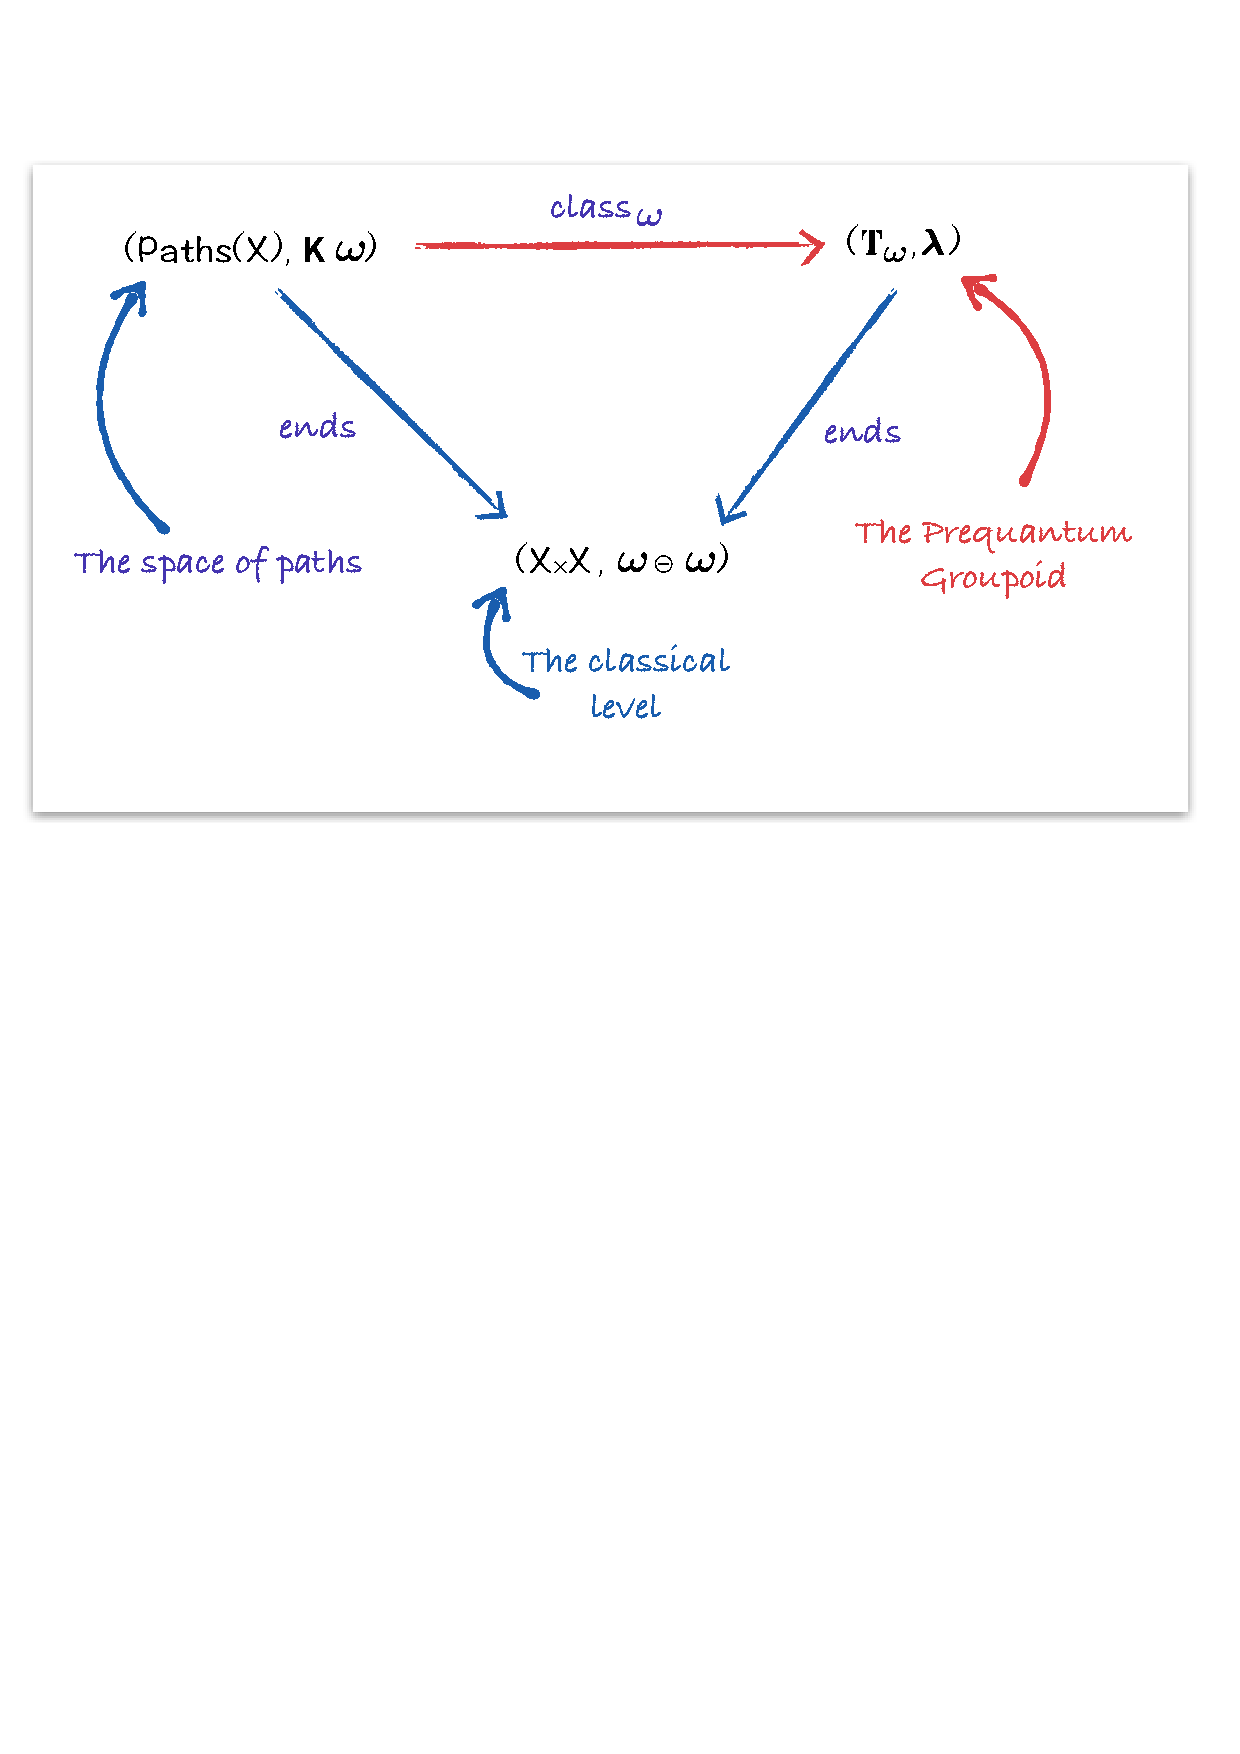
\includegraphics[width=0.75\textwidth]{Figures/Quantum-Groupoid-construct.pdf}
      \caption{\small\textbf{The Prequantum Reduction.}
      The diagram illustrates the construction of the prequantum groupoid $\TT_\omega$ as a quotient of the space of paths.
      The projection $\class_\omega$ descends the path-space 1-form $\Komega$ to the unique prequantum 1-form $\blambda$ on the groupoid.
      The curvature of $\blambda$ projects further to the difference of symplectic forms $\omega \ominus \omega$ on the space of endpoints $X \times X$.
      This structure identifies $\TT_\omega$ as the geometric object capturing the quantum phase information distilled from the paths.}
      \label{fig:reduction}
    \end{figure}
  \end{article}
  \begin{article}\artlabel[Structural Properties]
    The resulting object is a bona fide diffeological groupoid equipped with a connection.
    
    \begin{theorem}[The Quantum System]
      The groupoid $\TT_\omega$ satisfies the following structural properties.
      \begin{enumerate}
        \item It is a fibrating diffeological groupoid over $X$,
        meaning that the projection $\ends : \cY \to X \times X$ is a subduction.
        \item The isotropy group at any point $x$, $\TT_{\omega, x}$, is isomorphic to the torus of periods $\Tomega$.
        \item There exists a unique left-right invariant $1$-form $\blambda$ on $\cY$,
        the \emph{prequantum $1$-form},
        such that $\class_\omega^*(\blambda) = \Komega$.
        \item The curvature relates to the parasymplectic form by $d\blambda = \trg^*(\omega) - \src^*(\omega)$.
      \end{enumerate}
    \end{theorem}
    
    \begin{proof}
      The proof follows the lines of the simply connected case (Part I),
      with the crucial adaptation that the period group $\Pomega$ now accounts for the non-trivial homotopy.
      
      1.~\emph{Groupoid Structure.}
      The additivity of $\psi$ ensures that $\sim_\omega$ is compatible with concatenation.
      If $\gamma \sim_\omega \gamma_1$ and $\eta \sim_\omega \eta_1$,
      then the difference $\Phi(\gamma \vee \eta, \gamma_1 \vee \eta_1)$ decomposes into sums of $\Phi$ terms that vanish.
      
      2.~\emph{Isotropy.}
      The isotropy at $x_0$ is the set of loops $[\ell]_\omega$ such that $\Phi(\ell, \hat{x}_0) = 0$,
      which means $\psi(\ell) = 0$.
      Thus,
      $\TT_{\omega, x_0} \simeq \ker(\psi) \backslash \Loops(X, x_0) \simeq \Tomega$.
      Since $X$ is connected,
      all isotropy groups are isomorphic.
      
      3.~\emph{The Form $\blambda$.}
      The relation $\gamma \sim_\omega \gamma'$ implies $\int_\gamma^{\gamma'} \Komega \in \Pomega$.
      Locally,
      this means $\Komega$ descends to the quotient $\cY$ just as in the simply connected case.
      The invariance and curvature properties follow from the properties of the chain-homotopy operator $\CHO$.
    \end{proof}
  \end{article}
  
  \begin{article}\artlabel[Uniqueness and Classification]
    \label{art: Classification}
    
    The construction described in the previous articles yields a specific,
    canonical prequantum groupoid $\TT_\omega$ associated with the form $\omega$.
    Since the construction relies on the canonical 1-form $\Komega$,
    this groupoid is unique up to a canonical isomorphism (a change of base loops corresponds to a gauge transformation).
    
    However,
    one may ask if there exist \emph{other} prequantum groupoids over $X$ with the same curvature $\omega$ that are \emph{not} isomorphic to $\TT_\omega$.
    A prequantum groupoid is generally defined as a fibrating groupoid over $X$ with fiber $\Tomega$ equipped with a connection 1-form $\blambda'$ satisfying $d\blambda' = \trg^*\omega - \src^*\omega$.
    
    Following the classification established in \cite{PIZ95} for generalized prequantum fiber bundles,
    the set of isomorphism classes of such structures is not trivial.
    Any two prequantum groupoids $\TT$ and $\TT'$ with the same curvature differ by a "flat" structure,
    which corresponds to a character of the fundamental group $\chi \in \Hom(\pi_1(X), \Tomega)$.
    
    Specifically, the groupoid $\TT_\omega$ constructed here corresponds to the trivial character.
    Other non-isomorphic groupoids can be obtained by "twisting" $\TT_\omega$ with a character $\chi$ that cannot be lifted to $\RR$ (i.e., it is not the period of a closed 1-form).
    
    This leads to the general classification theorem, generalizing the result on fiber bundles to the groupoid context:
    
    \begin{theorem}[Classification]
      The set of isomorphism classes of prequantum groupoids with curvature $\omega$ is an affine space modeled on the group of characters $H^1(X, \Tomega)$.
      Modulo the gauge transformations induced by Hamiltonian automorphisms (exact 1-forms),
      the moduli space of prequantum structures is canonically identified with the extension group:
      $$
        \mathcal{M}(X, \omega) \simeq \Ext(\pi_1(X)^{\mathrm{ab}}, \Pomega).
        $$
    \end{theorem}
    
    Our path-based construction $\TT_\omega$ provides the canonical origin (the zero element) of this moduli space.
  \end{article}
  
  %%%%%%%%%%%%%%%%%%%%%%%%%%%%%%%%%%%%%%%%%%%%%%%%%%%%%%%%%%
  %% MARK: Section IV: Symmetries of the Quantum System
  %%%%%%%%%%%%%%%%%%%%%%%%%%%%%%%%%%%%%%%%%%%%%%%%%%%%%%%%%%
  
  \section{\textsc{\textbf{Symmetries of the Quantum System}}}
  \label{sec:Symmetries}
  
  We now address the symmetries of this structure.
  The result mirrors the simply connected case,
  demonstrating the robustness of the path-space construction against homotopic complexity.
  
  \begin{article}\artlabel[The Automorphism Group]
    Let $\Aut(\TT_\omega, \blambda)$ be the group of automorphisms of the groupoid $\TT_\omega$ that preserve the prequantum form $\blambda$.
    Let $\Diff(X, \omega)$ be the group of parasymplectic diffeomorphisms of $X$.
    
    \begin{theorem}[Full and Faithfull Symmetries]
      The projection $\pi: \Aut(\TT_\omega, \blambda) \to \Diff(X, \omega)$,
      defined by restricting the automorphism to the space of objects,
      is an isomorphism of diffeological groups.
      $$
        \Aut(\TT_\omega, \blambda) \simeq \Diff(X, \omega).
        $$
    \end{theorem}
  \end{article}
  
  \begin{proof}
    Let us begin by proving the surjectivity of $\pi$\/:
    
    1.~\emph{Surjectivity.}
    Let $g \in \Diff(X, \omega)$.
    The map $g$ acts on $\Paths(X)$ by composition: $\gamma \mapsto g \circ \gamma$.
    Since $g^*\omega = \omega$,
    the chain-homotopy operator satisfies $g^*(\Komega) = \Komega$.
    Consequently,
    integrals of $\Komega$ are preserved.
    This implies that $g$ preserves the set of periods $\Pomega$ (all spherical, toric, and surfacic periods are geometric invariants of $\omega$).
    Thus,
    if $\gamma \sim_\omega \gamma'$,
    then $g \circ \gamma \sim_\omega g \circ \gamma'$.
    The map descends to a well-defined automorphism $h$ on $\cY$.
    Since $\class_\omega^*(h^*\blambda) = (\class_\omega \circ g)^*(\blambda) = g^*(\class_\omega^*(\blambda)) = g^*(\Komega) = \Komega = \class_\omega^*(\blambda)$,
    and $\class_\omega$ is a subduction,
    we have $h^*\blambda = \blambda$.
    
    And then,
    the injectivity:
    
    2.~\emph{Injectivity.}
    Let $h$ be an automorphism of $\TT_\omega$ covering the identity on $X$.
    Then for any morphism $y \in \cY$,
    $h(y)$ can be written as $h(y) = \sigma(\src(y)) \cdot y$ for some section $\sigma: X \to \TT_\omega$,
    where $\sigma(x) \in \TT_{\omega,x}$ for each $x$.
    The condition that $h$ preserves the prequantum form,
    $h^*\blambda = \blambda$,
    implies that the section $\sigma$ is locally constant (its derivative must vanish).
    Since $X$ is connected,
    $\sigma$ must be a constant section.
    
    Furthermore,
    as an automorphism,
    $h$ must preserve the identity morphisms.
    Let $\id_x = \class_\omega(\hat{x}) \in \cY$ be the identity morphism at $x$.
    Then $h(\id_x) = \id_x$.
    Applying our formula,
    we get:
    $$
      h(\id_x) = \sigma(\src(\id_x)) \cdot \id_x = \sigma(x) \cdot \id_x = \sigma(x).
      $$
    Therefore,
    we must have $\sigma(x) = \id_x$ for all $x \in X$.
    
    This means the section $\sigma$ is the identity section.
    It follows that for any $y \in \cY$:
    $$
      h(y) = \sigma(\src(y)) \cdot y = \id_{\src(y)} \cdot y = y.
      $$
    Thus,
    $h$ is the identity automorphism on $\cY$,
    and the projection is injective.
  \end{proof}
  
  \begin{article}\artlabel[The Quantum Moment Map]
    The existence of the invariant form $\blambda$ allows for the definition of an equivariant moment map $\Psi$ on the prequantum groupoid $\TT_\omega$,
    for the action of the symmetry group $G_\omega = \Aut(\TT_\omega, \blambda) \simeq \Diff(X, \omega)$.
    Explicitly,
    $\Psi : \cY \to \cG_\omega^*$,
    where $\cG_\omega^*$ is the dual of the Lie algebra of $G_\omega$,
    is given by:
    $$
      \Psi(y) = \hat y^*(\blambda),
      $$
    where $\hat y: G_\omega \to \cY$ is the orbit map $\hat y(g) = g(y)$ \cite{PIZ10}.
    
    This map corresponds to the descent of the "paths moment map" $\Psi_{\paths}$ defined in \cite{PIZ10} to the quotient $\cY$.
    The restriction of $\Psi$ to the isotropy groups $\TT_{\omega, x} \simeq \Tomega$ captures the \emph{holonomy} of the system.
    If the holonomy is non-trivial,
    the moment map cannot descend to a single-valued function on $X$.
    However,
    it remains a well-defined,
    single-valued function on the Quantum System $\TT_\omega$.
    This resolves the apparent conflict with Souriau's principle for systems like the Aharonov-Bohm effect:
    the moment map exists,
    but its domain is the quantum groupoid,
    not the classical space.
  \end{article}
  
  \begin{article}\artlabel[The Holonomy and Souriau's Principle]
    This construction sheds new light on the theory of moment maps in diffeology.
    In \cite{PIZ10},
    we identified the \emph{holonomy group} $\Gamma = \Psi_{\text{paths}}(\Loops(X))$ as the obstruction for the moment map to descend to the space of motions $X$.
    
    We can now identify $\Psi_{\text{paths}}$ as the intrinsic moment map of the \emph{Quantum System} (the groupoid $\TT_\omega$).
    The condition $\Gamma = \{0\}$ corresponds to the principle of the existence of the moment map,
    which Souriau posited as essential for a system to constitute a "Dynamical System" in the strict sense (see \cite[p.161]{Sou70}).
    
    \begin{figure}[ht]
      \newcommand{\TL}{\Paths(X) \arrow[rr,"\Psi_\paths"] \arrow[dr, "\class_\omega"] \arrow[ddr, swap, "\ends"]}
      \newcommand{\TR}{\cG_\omega^* \arrow[dd,"\pr_\Gamma"]}
      \newcommand{\DM}{\cY \arrow[d,"\ends"] \arrow[ur,"\Psi_\omega"]}
      \newcommand{\BM}{X \times X \arrow[r, swap, "\psi_\omega"]}
      \newcommand{\BR}{\cG_\omega^*/\Gamma_\omega}
      \begin{center}
        \begin{tikzcd}[column sep=large, row sep=large, every label/.append style = {font = \small}]
          \TL  &  {}  & \TR   \\
          {}   & \DM  & {}     \\
          {}   & \BM  & \BR
        \end{tikzcd}
      \end{center}
      \caption{\small\textbf{The Factorization of the Moment Map.}
      The diagram illustrates how the moment map $\Psi_{\text{paths}}$,
      defined on the space of paths,
      descends to the prequantum groupoid $\cY$.
      The map $\Psi_\omega$ represents the intrinsic moment map of the Quantum System.
      The further descent to the classical space of motions $X \times X$ is obstructed by the holonomy group $\Gamma_\omega$.
      The projection $\pr_\Gamma$ indicates that on the classical Skeleton,
      the moment map is only defined modulo the quantum holonomy $\Gamma_\omega$,
      recovering Souriau's multivaluedness for "non-true" physical systems.}
    \end{figure}
    
    
    Systems with $\Gamma \neq \{0\}$,
    such as the Aharonov-Bohm effect,
    violate this classical principle:
    their dynamical quantities (momenta) are well-defined only on the prequantum groupoid $\TT_\omega$,
    not on the classical Skeleton $X$.
    The groupoid framework resolves this paradox:
    the moment map $\Psi_\omega$ exists and is single-valued,
    but its domain is the Quantum System $\TT_\omega$,
    not the classical space $X$.
    The Aharonov-Bohm effect is thus identified as a strictly quantum phenomenon captured by the intrinsic geometry of the groupoid,
    vindicating Souriau's principle by lifting it to the correct geometric arena
  \end{article}
  
  
  %%%%%%%%%%%%%%%%%%%%%%%%%%%%%%%%%%%%%%%%%%%%%%%%%%%%%%%%%%
  %% MARK: Section V: A Reconstruction of the Dirac Program
  %%%%%%%%%%%%%%%%%%%%%%%%%%%%%%%%%%%%%%%%%%%%%%%%%%%%%%%%%%
  
  \section{\textsc{\textbf{A Reconstruction of the Dirac Program}}}
  \label{sec:DiracProgram}
  
  The structural rigidity of the prequantum groupoid suggests a significant reorientation of the geometric quantization program.
  Classically,
  the quantization of symmetries is viewed as a reconstruction problem:
  given a group $G$ acting on $(X, \omega)$,
  one seeks to construct a unitary representation of $G$ on a Hilbert space.
  This process is often plagued by obstructions,
  requiring central extensions or metaplectic corrections at the very outset.
  
  Our framework offers a different paradigm.
  Since the group of automorphisms of the prequantum groupoid coincides with $\Diff(X, \omega)$,
  we possess \emph{ab initio} a canonical,
  linear,
  and faithful representation of the entire symmetry group.
  
  \begin{article}\artlabel[The Quantum System]
    We propose to define the \emph{Quantum System} as the pair $(\TT_\omega, \blambda)$,
    unique as the reduction of $(\Paths(X),\Komega)$.
    The space $X$ is embedded as the Skeleton of units $\Obj(\TT_\omega) \subset \Mor(\TT_\omega)$.
    The non-unit morphisms appear as a Quantum Fog surrounding the Skeleton of classical motions,
    if we regard $X$ as the space of motions of a dynamical system.
    A remarkable benefit of this path-based construction is that the symmetries of the classical system become,
    exactly and without modification,
    the symmetries of the Quantum System:
    we have only one system.
    
    In this view,
    quantization is not a process of \emph{synthesis} (building a representation),
    but a process of \emph{selection} (polarization).
    We select a subspace of multiplicative functions on $\TT_\omega$ (the wave functions) determined by a polarization.
    The "quantum anomalies" arise solely because the symmetry group does not preserve this selection.
    They are not defects of the prequantum geometry,
    but the necessary geometric cost of projecting the universal symmetry onto a specific observational framework.
    
    \textbf{Remark.}~(Dirac via Feynman).
    This construction revisits the Dirac quantization program in conformity with Feynman's perspective.
    The prequantum groupoid $\TT_\omega$ should be viewed as a \emph{condensed} space of paths that preserves the quantum 1-form and the symmetries of the system.
    The projection $\class_\omega$ is equivariant,
    intertwining the raw action on histories with the quantum action on morphisms,
    as well as relating the potential $\Komega$ with $\blambda$.
    Thus,
    the space of paths still stands over the groupoid; it is not discarded.
    
  \end{article}
  
  \begin{article}\artlabel[Derivation of the Dirac Axioms]
    In the case where $X$ is a smooth symplectic manifold, we can verify that this construction satisfies the historical Dirac axioms for quantization.
    
    1.~\emph{The Identity.}
    The constant function $u = \mathbf{1}$ generates the zero vector field $\xi_{\mathbf{1}} = 0$.
    The corresponding flow is the identity $\id_X$.
    The unique lift to the groupoid is $\id_{\TT_\omega}$.
    Thus,
    the operator associated with the constant function is strictly the identity operator.
    
    2.~\emph{The Commutator.}
    Let $u, v \in C^\infty(X)$.
    Their Hamiltonian vector fields $\xi_u, \xi_v$ lift uniquely to vector fields $\tilde\xi_u, \tilde\xi_v$ on $\TT_\omega$ preserving $\blambda$.
    The quantum operator is defined as $\hat{u} = i\hbar \tilde\xi_u$.
    A direct computation of the Lie bracket on the groupoid yields:
    $$
      [\hat{u}, \hat{v}] = [i\hbar \tilde\xi_u, i\hbar \tilde\xi_v] = -\hbar^2 [\tilde\xi_u, \tilde\xi_v] = -\hbar^2 (-\tilde\xi_{\{u,v\}}) = -i\hbar \widehat{\{u,v\}}.
      $$
    Thus,
    the Dirac commutator relation is derived directly from the geometry of the groupoid.
    
    \textbf{Remark.}~(The General Case).
    For general diffeological spaces, where tangent spaces may be ill-defined%
    \footnote{As recently demonstrated by Taho \cite{Tah25},
    there exist infinitely many non-isomorphic tangent functors on diffeological spaces extending the classical definition for manifolds.
    This lack of a unique canonical tangent structure reinforces the necessity of a covariant approach that avoids reliance on tangent vectors.}
    or the Poisson algebra of functions unavailable, the Poisson structure is understood \emph{covariantly}.
    As detailed in \cite{PIZ25},
    the Poisson bracket is defined via the orbit map of the symmetry group into the space of $2$-momenta,
    that is,
    the space of left invariant $2$-form.
    The isomorphism $\Aut(\TT_\omega, \blambda) \simeq \Diff(X, \omega)$ ensures that this covariant Poisson structure is faithfully represented by the quantum system,
    extending the correspondence principle beyond the scope of manifolds.
  \end{article}
  
  %%%%%%%%%%%%%%%%%%%%%%%%%%%%%%%%%%%%%%%%%%%%%%%%%%%%%%%%%%
  %% MARK: Section VI: Examples
  %%%%%%%%%%%%%%%%%%%%%%%%%%%%%%%%%%%%%%%%%%%%%%%%%%%%%%%%%%
  
  \section{\textsc{\textbf{Examples}}}
  \label{sec:Examples}
  
  We illustrate the construction of the prequantum groupoid through a series of examples ranging from exact symplectic structures to those with irrational periods and flat connections.
  These examples demonstrate how the groupoid framework unifies cases that are treated disparately in standard geometric quantization.
  
  \subsection*{A. The Exact Cases (Trivial Groupoid, Non-Trivial Holonomy)}
  
  When the parasymplectic form $\omega$ is exact,
  the group of periods is trivial,
  yet the homotopy of the space is preserved in the holonomy of the groupoid.
  
  \begin{article}\artlabel[The Punctured Plane]
    Let $X = \RR^2 - \{0\}$ equipped with the form $\omega = \frac{dx \wedge dy}{x^2 + y^2}$.
    In polar coordinates,
    $\omega = d(\log(r) d\theta)$.
    Despite the non-trivial fundamental group $\pi_1(X) \simeq \ZZ$,
    the form is exact globally.
    Consequently,
    the group of periods is trivial:
    $$
      \Pomega = \{0\} \qtext{and} \Tomega = \RR.
      $$
    The prequantum groupoid is the trivial additive groupoid $\TT_\omega \simeq X \times \RR \times X$.
    However,
    the holonomy is non-trivial:
    a loop $\gamma$ at radius $r$ accumulates an action $A(\gamma) = \int_\gamma \log(r) d\theta$.
    Two loops at different radii correspond to distinct morphisms in the groupoid,
    distinguishing the "magnetic" geometry even in the absence of quantized periods.
  \end{article}
  
  \begin{article}\artlabel[The Plane with Two Holes]
    Let $X = \RR^2 - \{p_1, p_2\}$.
    The fundamental group is the free group on two generators,
    $\pi_1(X) \simeq \langle a, b \rangle$.
    Since $X$ is an open surface,
    $H^2(X, \RR) = 0$,
    and any closed 2-form $\omega$ is exact.
    Thus,
    $\Pomega = \{0\}$.
    
    This example confirms that a complex homotopy (non-abelian $\pi_1$) does not force a non-trivial isotropy group.
    The prequantum bundle is trivial ($\RR$-fibers).
    The geometrical complexity is entirely encoded in the values of the action (the holonomy) on the free group,
    not in the curvature of the bundle.
  \end{article}
  
  \subsection*{B. The Compact Cases (Discrete Periods)}
  
  These are the standard cases of geometric quantization where the geometry forces the quantization of periods.
  
  \begin{article}\artlabel[The Torus $T^2$]
    Let $X = \RR^2/\ZZ^2$ equipped with the standard symplectic form $\omega = dx \wedge dy$.
    As calculated in Section \ref{sec:GroupAndTorusOfPeriods},
    the group of toric periods is $\Ptor = \ZZ$.
    The torus of toric periods is $\Ttor = \RR/\ZZ$.
    
    The fundamental group is $\pi_1(X) \simeq \ZZ^2$.
    The fundamental relation defining the torus is the commutator $ABA^{-1}B^{-1} = 1$,
    where $A$ and $B$ are the generators of the lattice.
    
    The "Surfacic Period" associated with this relation is the integral of $\omega$ over the surface bounded by the commutator loop.
    Geometrically,
    this corresponds to the total area of the fundamental domain:
    $$
      \int_{\text{fund. domain}} \omega = \text{Area}(T^2) = 1.
      $$
    Therefore,
    $\Pomega$ must contain both the toric periods ($\ZZ$) and the total area ($1$).
    In this standard case,
    they coincide:
    $$
      \Pomega = \Ptor = \ZZ.
      $$
    The prequantum isotropy is $\RR/\ZZ$,
    recovering the standard prequantization of the torus.
  \end{article}
  
  \begin{article}\artlabel[Surface of Genus $g>1$]
    Let $\Sigma_g$ be a compact surface of genus $g > 1$ with area form $\omega$.
    Since $\pi_2(\Sigma_g) = 0$,
    $\Psph = \{0\}$.
    Also,
    since there are no non-contractible tori in $\Sigma_g$ for $g>1$,
    $\Ptor = \{0\}$ and $\Ttor = \RR$.
    
    The total periods must therefore come entirely from the surfacic cocycle $\tau$.
    Consider the loop $\gamma_R$ representing the fundamental relation $R = \prod [a_k, b_k]$ (the boundary of the fundamental polygon).
    
    Geometrically,
    the integral of $\Komega$ along this relation represents the total area of the surface.
    Algebraically,
    this value is generated by the cocycle $\tau$ evaluated on the commutators.
    Therefore:
    $$
      \Pomega = \text{Area}(\Sigma_g) \cdot \ZZ.
      $$
    The prequantum isotropy group is $\TT_{\omega,x} \simeq \RR / (\text{Area}(\Sigma_g)\cdot\ZZ)$.
    This illustrates the necessity of the surfacic cocycle:
    here $\Ptor$ was zero,
    yet $\Pomega$ is non-trivial.
  \end{article}
  
  \subsection*{C. The General Cases (Irrational and Flat)}
  
  These examples highlight the unique power of the diffeological framework.
  
  \begin{article}\artlabel[Composite Systems and Irrational Periods]
    Let us consider a composite system formed by two independent elementary systems.
    For instance,
    let $X = S^2 \times S^2$,
    equipped with the product symplectic form:
    $$
      \omega = s_1\omega_1 \oplus s_2 \omega_2 = \pr_1^*(s_1\surf_{S^2}) + s_2 \pr_2^*(\surf_{S^2}),
      $$
    where $\surf_{S^2}$ is the standard area form on the sphere normalized such that $\int_{S^2} \surf_{S^2} = 1$,
    and $s_1, s_2\in \RR$ are the coupling constants.
    
    The space $X$ is simply connected.
    The group of periods is generated by the spherical periods of the two factors (elements of $\pi_2(X) \simeq \ZZ \oplus \ZZ$).
    Thus:
    $$
      \Pomega = \left\{ n s_1 + m s_2 \mid n,m \in \ZZ \right\} = s_1 \ZZ + s_2\ZZ.
      $$
    The nature of the prequantum isotropy depends crucially on the rationality of $\alpha = s_2/s_1$, the ratio of scales.
    
    1.~\emph{The Rational Case.}
    If $\alpha \in \QQ$,
    say $\alpha = p/q$,
    then $\Pomega = \frac{1}{q}\ZZ$.
    The group of periods is discrete and isomorphic to $\ZZ$.
    The torus of periods $\Tomega \simeq \RR/\frac{1}{q}\ZZ$ is a circle.
    This recovers the standard case where the system admits a prequantum line bundle.
    
    2.~\emph{The Irrational Case.}
    If $\alpha \notin \QQ$,
    the group $\Pomega$ is a dense subgroup of $\RR$.
    In the classical framework of geometric quantization,
    this system is considered "non-quantizable" because no principal bundle with structure group $\U(1)$ exists with curvature $\omega$.
    However,
    in our diffeological framework,
    the prequantum groupoid $\TT_\omega$ is perfectly well-defined.
    The isotropy group is the \emph{irrational torus}:
    $$
      \Tomega = \RR / (\ZZ + \alpha\ZZ).
      $$
    This space is a "bad" quotient in topology (non-Hausdorff),
    but a standard and well-behaved object in diffeology (the model of the irrational flow on the torus).
    
    This example demonstrates that the "integrality condition" of Kostant-Souriau is not a condition for the \emph{existence} of the prequantum geometry,
    but rather a condition for the quantum phase $\Tomega$ to be a smooth manifold.
    The diffeological prequantum groupoid captures the geometry of systems with incommensurable periods without obstruction,
    suggesting a generalized quantum mechanics where the phase factor lives in a generalized torus.
  \end{article}
  
  \begin{article}\artlabel[The Aharonov-Bohm Effect]
    Let $X = \RR^2 - \{0\}$ with $\omega = 0$.
    The canonical groupoid is trivial.
    However,
    the moduli space of prequantum structures is $H^1(X, \Tomega) \simeq \Tomega$.
    The Aharonov-Bohm system corresponds to a "flat" groupoid $\TT_{AB}$ with non-trivial holonomy determined by the flux $\Phi$:
    $$
      [\gamma]_{AB} = (\gamma(0), n\Phi, \gamma(0)).
      $$
    Jean-Marie Souriau noted that describing this effect with functions on the space of motions leads to multi-valued Hamiltonians or apparent conservation violations.
    Our framework resolves this:
    the Hamiltonian is well-defined and conserved,
    but it generates a flow on the non-trivial groupoid $\TT_{AB}$.
    The energy is preserved,
    but the geometric structure carrying it is twisted.
  \end{article}
  
  %%%%%%%%%%%%%%%%%%%%%%%%%%%%%%%%%%%%%%%%%%%%%%%%%%%%%%%%%%
  %% MARK: Section VII: Discussion
  %%%%%%%%%%%%%%%%%%%%%%%%%%%%%%%%%%%%%%%%%%%%%%%%%%%%%%%%%%
  
  \section{\textsc{\textbf{Discussion}}}
  \label{sec:Discussion}
  
  The construction of the prequantum groupoid $\TT_\omega$ presented here is valid for any connected parasymplectic space,
  regardless of the rationality of its periods or the categorical nature of the underlying diffeological space.
  It applies to manifolds,
  orbifolds,
  quasifolds,
  and infinite-dimensional spaces such as loop spaces or connections.
  This generality invites a re-evaluation of several standard concepts in geometric quantization.
  
  % ----- The Topological Blind Spot -----
  \subsection*{The Topological Blind Spot}
  This construction highlights a fundamental epistemological rupture with standard geometric quantization.
  Historically,
  quantization relied on Chern-Weil theory,
  governed by topological invariants (Chern classes).
  This created a "blind spot":
  for spaces with coarse topology (like the irrational torus or leaf spaces of foliations),
  topological tools detected no structure,
  leading to the conclusion of non-quantizability.
  
  Our result demonstrates that the obstruction was in the category used,
  not the geometry.
  Diffeology succeeds where topology fails because it defines the fundamental group and periods via \emph{smooth probes} (plots),
  not open sets.
  For the irrational torus,
  topology sees a point,
  but Diffeology sees the dense winding ($\pi_1 \simeq \ZZ^2$),
  allowing a non-trivial prequantum groupoid.
  Thus,
  the condition for quantization is not topological non-triviality,
  but \emph{diffeological discreteness} of the group of periods.
  
  % ----- The Geometric Alternative to Path Integration -----
  \subsection*{The Geometric Alternative to Path Integration}
  The path-based nature of our construction suggests a deep connection to Feynman's path integral formulation,
  but with a radical shift in perspective.
  In the Feynman approach,
  one sums amplitudes over all paths,
  relying on the principle that paths with action differences in $h\ZZ$ interfere constructively.
  
  In our diffeological framework,
  we replace this analytic summation with a geometric quotient.
  The equivalence relation $\sim_\omega$ identifies precisely those paths that would interfere constructively.
  By taking the quotient,
  we do not destroy the quantum information;
  we \emph{distill} it.
  This process eliminates the redundant "history" of the motion,
  leaving only the \emph{freedom for interference}:
  the quantum phase itself.
  
  The Prequantum Groupoid $\TT_\omega$ can thus be viewed as the \emph{geometric crystallization} of the path integral:
  it is the structure that remains once the constructive interference has been geometrically resolved.
  
  \subsection*{Lagrangian Perturbations and Quantum Fluctuations}
  To fully understand the physical meaning of paths in the space of motions,
  we must revisit the origins of symplectic calculus by Lagrange \cite{PIZ98}.
  Lagrange described the motion of a perturbed system as a curve in the space of unperturbed motions
  (originally, the space of Keplerian elements).
  
  In the language of Souriau,
  consider a system defined by an "analytical system" associated with identified forces.
  The evolution space $Y$ is equipped with a presymplectic form $\varpi$,
  and the space of motions is the quotient $X = Y/\ker(\varpi)$.
  Any virtual path of the particle $t \mapsto r(t)$ in configuration space lifts to a path $t \mapsto y(t) = (r(t), \dot r(t), t)$ in $Y$,
  which in turn projects to a path $\gamma: t \mapsto x(t)$ in the space of motions $X$.
  
  Following Lagrange,
  this path $\gamma$ represents a \emph{perturbed motion}:
  a continuous variation of the constants of motion.
  In our framework,
  we interpret quantum phenomena as subtle,
  non-analytical,
  fuzzy perturbations that manifest as finite variations in the space of motions.
  The prequantum groupoid $\TT_\omega$ acts as a filter for these variations.
  It retains only the symplectic phase information defined by $\omega$.
  
  Thus,
  each arrow in the groupoid represents a possible transition from one regular motion to another under this indescribable,
  fuzzy perturbation that we call \emph{quantum fluctuation}.
  This reconciles Feynman's original consideration of virtual paths with the symplectic geometry of Lagrange,
  condensing unpredictable perturbations into precise quantum transitions.
  
  % ----- Relation to Other Frameworks -----
  \subsection*{Relation to Other Frameworks}
  The use of groupoids and path spaces in quantization has a rich history,
  and it is useful to situate our construction within this landscape.
  Weinstein and Karasev introduced symplectic groupoids to integrate Poisson manifolds \cite{Wei87, Kar87},
  where prequantization typically involves constructing a bundle over the groupoid.
  Brylinski and others explored the geometry of the loop space and the transgression of the 3-form to define prequantum structures in infinite dimensions \cite{Bry93}.
  More recently,
  the language of gerbes and stacks has been employed to address topological obstructions and non-integrality \cite{Mur96}.
  
  Our approach differs by remaining strictly within the framework of geometry (a.k.a. diffeology).
  Instead of moving to higher categorical structures (stacks) or remaining in the unreduced space of loops,
  we construct a prequantum object directly over the base space,
  reducing the path space to the intrinsic degrees of freedom of the system.
  Diffeology allows us to treat the resulting quotients (whether singular,
  irrational,
  or infinite-dimensional) as valid geometric spaces,
  incorporating non-integral periods as intrinsic features of the geometry rather than obstructions requiring a change of category.
  
  % ----- The Intrinsic Decomposition of Periods -----
  \subsection*{The Intrinsic Decomposition of Periods}
  The definition of the Total Group of Periods $\Pomega$ offers an intrinsic decomposition of the symplectic action, independent of external homological machinery.
  Standard quantization often imports the second homology group $H_2(X, \ZZ)$ as a topological datum to define periods.
  Our construction "disarticulates" the period group into three geometric components strictly internal to the homotopy of the path space:
  \begin{enumerate}
    \item \textbf{Spherical Periods} ($\Psph$): Arising from contractible loops (genus 0 bubbles).
    \item \textbf{Toric Periods} ($\Ptor$): Arising from the geometry of the loop space components (genus 1 cylinders).
    \item \textbf{Surfacic Periods} ($\tau$): Arising from the non-commutativity of the fundamental group (genus $>1$ commutators).
  \end{enumerate}
  By generating $\Pomega$ from these sources, the path space reveals the "homological" constraints of the system without ever leaving the realm of smooth paths, adhering to the diffeological principle of minimal external construction.
  
  % ----- The Universality of the Quantum Unit -----
  \subsection*{The Universality of the Quantum Unit}
  This perspective extends naturally to the interaction between distinct systems.
  If we accept as a fundamental principle that any two quantum systems can interact to form a composite system,
  then their respective period groups must be commensurable.
  This requires a universal quantum unit of action,
  $h$ (Planck's constant),
  such that $Pomega \subseteq h\ZZ$ for all physically realizable systems.
  
  In this view,
  the "Universal Quantum Torus" is $\TT_{\quant} = \RR / h\ZZ$.
  The isomorphism between the geometric isotropy group $T_\omega = \RR/Pomega$ and the group of phases $\U(1)$ is mediated by the Planck constant $\hbar = h/2\pi$.
  
  % ----- The Wave Function as a Multiplicative Map -----
  \subsection*{The Wave Function as a Multiplicative Map}
  The identification of the groupoid as the quantum system suggests a natural,
  intrinsic definition for the wave function.
  In the standard bundle approach,
  a wave function is a section of a line-bundle,
  which requires a local trivialization and transition functions.
  
  In the groupoid framework,
  a quantum state is simply a smooth,
  complex-valued function $\Psi$ defined on the space of morphisms $\cY$ that is \emph{multiplicative}:
  $$
    \Psi(y \cdot y') = \Psi(y) \cdot \Psi(y').
    $$
  This condition enforces that $\Psi$ transforms according to a character of the isotropy group $\Tomega$ (the quantum phase).
  Specifically,
  for any loop $\tau \in \TT_{\omega, x}$,
  we have $\Psi(\tau \cdot y) = \chi(\tau)\Psi(y)$.
  This definition is covariant,
  requires no auxiliary choices (like open covers),
  and naturally accommodates the action of the symmetry group $\Diff(X, \omega)$ via pullback.
  
  % ----- Intrinsic Quantization of Reduced Spaces -----
  \subsection*{Intrinsic Quantization of Reduced Spaces}
  The diffeological framework resolves the debate regarding whether "quantization commutes with reduction."
  Our approach grants the reduced space an autonomous status.
  Once the reduction is performed,
  the quotient space $Q$ is a fully defined diffeological space.
  If the parasymplectic form descends to a closed 2-form $\omega$ on $Q$,
  we can apply our construction directly to $Q$.
  
  The reduced system is thus immediately "clothed" in its own prequantum structure.
  The unit map $x \mapsto \id_x$ embeds the classical space $X$ strictly into the space of morphisms of $\TT_\omega$.
  The classical space sits inside the prequantum groupoid like a sharp Skeleton,
  enveloped by the Quantum Fog of non-identity morphisms.
  In this view,
  quantization does not need to commute with reduction;
  rather,
  \emph{reduction defines the physical system,
  and quantization renders it quantum}.
  
  % ----- Elementary vs. Composite Systems -----
  \subsection*{Elementary vs. Composite Systems}
  The construction of the prequantum groupoid invites a re-evaluation of the notion of an ``elementary system.''
  Following the program of Souriau and Kostant,
  an elementary particle is traditionally defined as a symplectic manifold upon which a specific symmetry group (such as the Galilean or Poincaré group) acts transitively.
  However,
  as shown in \cite{DIZ22},
  every connected symplectic manifold is a coadjoint orbit of its own group of quantomorphisms (a central extension of the Hamiltonian group).
  Thus,
  transitivity alone,
  without specifying a restricted group \emph{a priori},
  is not a sufficient discriminator.
  
  The diffeological framework,
  particularly through the lens of the prequantum groupoid,
  suggests an intrinsic definition based on the \emph{natural} symmetries of the system.
  We have established that the group of automorphisms of the quantum system is isomorphic to $\Diff(X, \omega)$.
  We propose the following classification:
  
  \begin{enumerate}
    \item \textbf{Elementary Systems:} A parasymplectic space $(X, \omega)$ is elementary if the group $\Diff(X, \omega)$ acts transitively on $X$.
    In the language of the groupoid,
    the subspace of units (the Skeleton) constitutes a single orbit under the action of the automorphism group.
    This implies that the space $X$ consists of a single Klein stratum%
    \footnote{Klein stratum with respect to local automorphisms of the structure $(X,\omega)$.}
    (locally homogeneous).
    Examples include the sphere $S^2$,
    the projective plane $P^2(\CC)$,
    and affine symplectic spaces.
    
    \item \textbf{Composite Systems:} A system is composite if the action of $\Diff(X, \omega)$ is not transitive.
    This typically occurs when $X$ possesses a non-trivial Klein stratification.
    Since diffeomorphisms must preserve the local diffeological type,
    they cannot map points from one stratum to another.
    The Skeleton of the quantum system is thus partitioned into disjoint invariant sectors.
  \end{enumerate}
  
  This distinction resolves the ambiguity in the modeling of the Deuteron discussed in Part I.
  The smooth model $P^2(\CC)$ is elementary;
  its symmetry group acts transitively.
  The singular model $\Sigma_4 = (S^2 \times S^2)/\fS_2$ is composite;
  it possesses a singular stratum (the diagonal) distinct from the principal stratum.
  The group $\Diff(\Sigma_4, \omega_s)$ preserves this stratification and is therefore not transitive.
  The singularity is thus the geometric signature of the composite nature of the system,
  a feature that is lost in the smooth approximation.
  
  % ----- Singularities and the Constancy of the Phase -----
  \subsection*{Singularities and the Constancy of the Phase}
  This intrinsic construction clarifies the treatment of singularities.
  Alternative approaches often model prequantization on stratified spaces by allowing the fiber to degenerate.
  In our framework,
  because the groupoid is constructed from the global period group $\Pomega$,
  the isotropy group $T_\omega$ remains constant everywhere,
  even at singular points.
  
  This respects the physical intuition that the phase degree of freedom is a universal constant of the theory,
  not a local variable.
  The singularity of the reduced space is encoded in the rich structure of the groupoid morphisms (the paths),
  not in the degeneration of the fiber.
  
  Following the program of Dirac \cite{Dir30} and Souriau \cite{Sou70},
  we regard the space of motions as the primary physical reality.
  While Marsden and Weinstein \cite{MW74} provided a powerful tool for analyzing symmetries,
  the process of reduction can obscure the global geometry of the system,
  particularly in the presence of singularities \cite{SL91}.
  As demonstrated by the author's work on the geometry of geodesics \cite{PIZ19,PIZ25b},
  and in the spirit of the optical analogy in symplectic mechanics \cite{GS84} or Sternberg's general covariance \cite{Ste06},
  the space of motions often possesses a unified structure
  (such as the conformal co-symplectic structure)
  that is fragmented by reduction.
  Our diffeological construction preserves this unity,
  ensuring that the quantum phase---the "extra floor" required by Groenewold and Van Hove---remains a universal constant of the theory,
  rather than a variable dependent on the stratification.
  
  % ----- The Source and the Screen -----
  \subsection*{The Source and the Screen}
  We propose that the prequantum groupoid $\TT_\omega$ \emph{is} the Quantum System in its objective state.
  Polarization is analogous to placing a \emph{screen} or \emph{lens} on this Quantum Source.
  The "quantum anomalies" (central extensions, metaplectic signs) are artifacts of the screen,
  not defects of the source.
  The prequantum groupoid supports the full symmetry group $\Diff(X, \omega)$ faithfully,
  while a specific polarization may break this symmetry.
  
  \subsection*{The Geometric Alternative to Path Integration}
  The path-based nature of our construction suggests a deep connection to Feynman's path integral formulation.
  Feynman's method extracts the quantum signal by \emph{averaging over the noise} of infinite path fluctuations.
  Our method adopts the inverse strategy:
  we \emph{quotient out the noise}.
  The projection $\class_\omega: \Paths(X) \to \TT_\omega$ acts as a geometric filter,
  identifying all paths that carry the same phase information.
  
  The groupoid $\TT_\omega$ is thus the space of pure \emph{signals}.
  This suggests a geometric factorization of the path integral,
  separating the universal geometric phase (captured by the finite-dimensional groupoid) from the dynamical amplitude.
  
  % ----- The Intrinsic Action Principle -----
  \subsection*{The Intrinsic Action Principle}
  Souriau famously emphasized that not all dynamical systems admit a global Lagrangian or Action functional on the space of motions; the sphere $S^2$ is the archetypal example where the symplectic form is closed but not exact.
  Standard geometric quantization resolves this by constructing a prequantum bundle, effectively creating a space where a global potential exists.
  However, this construction can feel like an artificial addition of external data to the classical system.
  
  Our framework reveals that the "missing" action is actually present and intrinsic, provided one looks in the correct space.
  While $\omega$ may not admit a global primitive $\theta$ on $X$ (i.e., $\omega \neq d\theta$), the $1$-form $\Komega$ is \emph{always} globally defined on $\Paths(X)$.
  It serves as a canonical, intrinsic "action form" for any parasymplectic space.
  
  Thus, the pair $(\Paths(X), \Komega)$ recovers the universality of the action principle without the need to postulate a Lagrangian or construct an external bundle.
  The geometry of $\omega$ generates its own action automatically when lifted to the path space, reconciling Souriau's primacy of the symplectic form with the physicist's need for a global action principle.
  
  % ----- Quantization as Transmutation -----
  \subsection*{Quantization as Transmutation}
  Ultimately,
  this framework suggests that geometric quantization is the revelation of intrinsic relational geometry.
  The classical space of motions $X$ presents a static view where states are isolated points.
  The prequantum groupoid $\TT_\omega$ reveals the dynamic reality:
  it is the geometry of a system where motions are allowed to \emph{transmute} into one another.
  
  The morphisms of the groupoid are the \emph{channels} of these transmutations,
  operated through the "one-dimensional nerves" of the paths.
  In this view,
  the quantum phase is not an external variable;
  it is the measure of the symplectic area swept by these nerves during the transmutation.
  
  % ----- Mutual Relativity and the Groupoid -----
  \subsection*{Mutual Relativity and the Groupoid}
  The groupoid construction over $X \times X$ reflects \emph{mutual relativity}.
  Quantities like action or phase are relational,
  connecting states $x$ and $x'$,
  not attributes of a single state.
  The traditional approach of fixing a reference state $x_0$ breaks covariance and introduces artifacts via cohomology.
  Our groupoid $\TT_\omega$ avoids this by being purely additive and covariant,
  preserving the full symmetry group $\Diff(X, \omega)$ without central extensions.
  It is the geometry of pure relation.
  
  %%%%%%%%%%%%%%%%%%%%%%%%%%%%%%%%%%%%%%%%%%%%%%%%%%%%%%%%%%
  %%
  %% MARK: - Bibliography
  %%
  %%%%%%%%%%%%%%%%%%%%%%%%%%%%%%%%%%%%%%%%%%%%%%%%%%%%%%%%%%
  
  \begin{thebibliography}{99}
    
    \bibitem[Bry93]{Bry93}
    Jean-Luc Brylinski.
    \newblock {\em Loop Spaces, Characteristic Classes and Geometric Quantization}.
    \newblock Progress in Mathematics, Vol. 107. Birkhäuser Boston, 1993.
    
    \bibitem[Dir30]{Dir30}
    P. A. M. Dirac.
    \newblock {\em The Principles of Quantum Mechanics}.
    \newblock Oxford University Press, Oxford, 1st edition, 1930.
    \newblock (4th edition, 1958).
    
    \bibitem[DIZ22]{DIZ22}
    Paul Donato and Patrick Iglesias-Zemmour.
    \newblock Every symplectic manifold is a (linear) coadjoint orbit.
    \newblock {\em Canadian Mathematical Bulletin}, 65(2):345--360, 2022.
    \newblock doi:10.4153/S000843952100031X.
    
    \bibitem[GS84]{GS84}
    Victor Guillemin and Shlomo Sternberg.
    \newblock {\em Symplectic Techniques in Physics}.
    \newblock Cambridge University Press, Cambridge, 1984.
    
    \bibitem[Kar87]{Kar87}
    Mikhail V. Karasev.
    \newblock Analogues of objects of the theory of Lie groups for nonlinear Poisson brackets.
    \newblock {\em Math. USSR Izvestija}, 28:497--527, 1987.
    
    \bibitem[KM85]{KM85}
    M. I. Kargapolov and Ju. I. Merzljakov.
    \newblock {\em Fundamentals of the theory of groups}.
    \newblock Graduate Texts in Mathematics, vol. 62, Springer-Verlag, New York-Berlin, 1979.
    
    \bibitem[Mur96]{Mur96}
    Michael K. Murray.
    \newblock Bundle gerbes.
    \newblock {\em Journal of the London Mathematical Society}, 54(2):403--416, 1996.
    
    \bibitem[PIZ98]{PIZ98}
    Patrick Iglesias-Zemmour.
    \emph{Les origines du calcul symplectique chez Lagrange}.
    L'Enseignement Math\'ematique (2) \textbf{44} (1998), no. 3-4, 257--277.
    
    \bibitem[PIZ85]{PIZ85}
    Patrick Iglesias,
    \emph{Fibrations difféologiques et homotopie},
    D.Sc. Thesis, Université de Provence, Marseille, 1985.
    
    \bibitem[PIZ10]{PIZ10}
    Patrick Iglesias-Zemmour,
    \emph{The moment maps in diffeology},
    Mem. Amer. Math. Soc. \textbf{204} (2010), no. 962.
    
    \bibitem[PIZ13]{PIZ13}
    Patrick Iglesias-Zemmour.
    {\em Diffeology}.
    Mathematical Surveys and Monographs, 185, Am. Math. Soc., 2013.
    
    \bibitem[PIZ19]{PIZ19}
    Patrick Iglesias-Zemmour,
    \emph{Refraction and reflexion according to the principle of general covariance},
    Journal of Geometry and Physics,
    Volume 142,
    2019,
    Pages 1-8,
    ISSN 0393-0440,
    {\scriptsize\url{https://doi.org/10.1016/j.geomphys.2019.03.013}}.
    
    \bibitem[PIZ25]{PIZ25}
    \bysame,
    \emph{Lectures on Diffeology},
    Beijing World Publishing Corp., Beijing, 2025. ISBN: 978-7-5232-1841-9.
    
    \bibitem[PIZ25a]{PIZ25a}
    Patrick Iglesias-Zemmour.
    \emph{Geometric Quantization by Paths, Part I: The Simply Connected Case},
    (Preprint, 2025). Available at \url{https://arxiv.org/abs/2508.11337}.
    
    \bibitem[PIZ25b]{PIZ25b}
    Patrick Iglesias-Zemmour.
    \emph{A Conformal Co-symplectic Structure on the Space of Pseudo-Riemannian Geodesics},
    (Preprint, 2025).
    {\scriptsize\url{https://math.huji.ac.il/~piz/documents/ACCSSOSOPRG.pdf}}.
    
    \bibitem[PIZ95]{PIZ95}
    Patrick Iglesias.
    {\em La trilogie du moment}.
    Ann. Inst. Fourier, 45(3):825--857, 1995.
    
    \bibitem[MW74]{MW74}
    Jerrold E. Marsden and Alan Weinstein,
    \emph{Reduction of symplectic manifolds with symmetry},
    Rep. Mathematical Phys. \textbf{5} (1974), no. 1, 121--130.
    
    \bibitem[SL91]{SL91}
    Reyer Sjamaar and Eugene Lerman.
    \newblock {\em Stratified symplectic spaces and reduction}.
    \newblock Annals of Mathematics, 134(2):375--422, 1991.
    
    \bibitem[Sou70]{Sou70}
    Jean-Marie Souriau.
    {\em Structure des syst\`emes dynamiques}.
    Dunod, Paris, 1970.
    
    \bibitem[Ste06]{Ste06}
    Shlomo Sternberg.
    \newblock {\em General Covariance and the Passive Equations of Physics}.
    \newblock Albert Einstein Memorial Lectures. The Israel Academy of Sciences and Humanities, Jerusalem, 2006.
    \newblock ISBN 965-208-173-6.
    
    \bibitem[Tah25]{Tah25}
    Masaki Taho.
    \newblock {\em Infinitely Many Tangent Functors on Diffeological Spaces}.
    \newblock Preprint arXiv:2511.17871, 2025.
    
    \bibitem[Wei87]{Wei87}
    Alan Weinstein.
    \newblock Symplectic groupoids and Poisson manifolds.
    \newblock {\em Bulletin of the American Mathematical Society}, 16:101--104, 1987.
    
  \end{thebibliography}
  
  %%%%%%%%%%%%%%%%%%%%%%%%%%%%%%%%%%%%%%%%%%%%%%%%%%%%%%%%%%
  %%
  %% MARK: - End Document
  %%
  %%%%%%%%%%%%%%%%%%%%%%%%%%%%%%%%%%%%%%%%%%%%%%%%%%%%%%%%%%
  
  \end{document}
